%======================================================================
%  DriveShieldX -- Technical Paper Presentation (Beamer, 16:9)
%  Every sentence, number and reference is taken from the research paper:
%  "DriveShieldX: Smart Traffic Violation and Road Safety Monitoring
%   System Using YOLOv8, Centroid-Based Tracking, and Multi-Violation
%   Detection" -- H. Makwana, N. Mandal, T. Sankhe, S. Kadam
%  Style follows the department reference deck (SignBridge).
%  Compile with pdfLaTeX (Overleaf: Menu -> Compiler -> pdfLaTeX).
%======================================================================
\documentclass[aspectratio=169,10pt,t]{beamer}

%------------------------ Packages ------------------------------------
\usepackage[T1]{fontenc}
\usepackage[utf8]{inputenc}
\usepackage[scaled=0.95]{helvet}
\renewcommand{\familydefault}{\sfdefault}
\usepackage{amsmath,amssymb}
\usepackage{booktabs,tabularx,array,multirow,makecell}
\usepackage{tikz}
\usetikzlibrary{arrows.meta,positioning,shapes.geometric,shapes.multipart,fit,calc,backgrounds}
\usepackage{pgfplots}
\pgfplotsset{compat=1.18}

%------------------------ EDIT HERE: roll numbers ---------------------
% Roll numbers (they appear on the title and
% acknowledgement slides).
\newcommand{\rollHeli}{44}
\newcommand{\rollNisha}{45}
\newcommand{\rollTanisha}{65}

%------------------------ Colours (same as reference deck) ------------
\definecolor{dsblue}{rgb}{0.2,0.2,0.7}      % header bar / headings
\definecolor{dsfoot}{RGB}{20,20,20}         % footer bar
\definecolor{dsred}{RGB}{200,30,30}         % "not measured" (as in paper)
\definecolor{sBlue}{HTML}{2a78d6}           % chart series 1
\definecolor{sOrange}{HTML}{eb6834}         % chart series 2
% architecture-figure fills (as in paper Fig. 1)
\definecolor{fGreen}{RGB}{220,250,220}  \definecolor{dGreen}{RGB}{20,130,20}
\definecolor{fOrange}{RGB}{253,238,222} \definecolor{dOrange}{RGB}{190,95,0}
\definecolor{fRed}{RGB}{253,225,230}    \definecolor{dRed}{RGB}{180,20,30}
\definecolor{fBlue}{RGB}{228,228,252}   \definecolor{dBlue}{RGB}{30,30,150}
\definecolor{fYellow}{RGB}{255,250,190} \definecolor{fGray}{RGB}{240,240,240}

%------------------------ Beamer look (matches reference) -------------
\setbeamertemplate{navigation symbols}{}
\setbeamercolor{structure}{fg=dsblue}
\setbeamercolor{normal text}{fg=black}
\setbeamercolor{alerted text}{fg=dsblue}
\setbeamercolor{frametitle}{bg=dsblue,fg=white}
\setbeamerfont{frametitle}{size=\Large}
\setbeamertemplate{frametitle}{%
  \nointerlineskip
  \begin{beamercolorbox}[wd=\paperwidth,ht=3.7ex,dp=1.6ex,leftskip=0.9em]{frametitle}%
    \usebeamerfont{frametitle}\insertframetitle
  \end{beamercolorbox}\vspace{0.2ex}}
\setbeamercolor{footbar}{bg=dsfoot,fg=white}
\setbeamertemplate{footline}{%
  \begin{beamercolorbox}[wd=\paperwidth,ht=2.4ex,dp=1.0ex]{footbar}%
    \hspace*{2.5em}\hfill\scriptsize COMPUTER SCIENCE AND TECHNOLOGY\hfill
    \makebox[2.5em][r]{\scriptsize\insertframenumber}\hspace*{0.8em}%
  \end{beamercolorbox}}
\setbeamertemplate{itemize item}{\small\raise0.15ex\hbox{\color{dsblue}$\blacktriangleright$}}
\setbeamertemplate{itemize subitem}{\scriptsize\raise0.2ex\hbox{\color{dsblue}$\blacktriangleright$}}
\setbeamertemplate{enumerate item}{\color{dsblue}\insertenumlabel.}
\setbeamertemplate{enumerate subitem}{\color{dsblue}\insertsubenumlabel)}
\setbeamersize{text margin left=1.6em,text margin right=1.6em}
% blocks (used for the 3-block literature survey etc.)
\setbeamertemplate{blocks}[rounded][shadow=false]
\setbeamercolor{block title}{bg=dsblue,fg=white}
\setbeamercolor{block body}{bg=dsblue!6,fg=black}
\setbeamerfont{block title}{size=\footnotesize,series=\bfseries}

%------------------------ Helpers -------------------------------------
\newcommand{\hd}[1]{{\color{dsblue}\textbf{#1}}}          % blue sub-heading
\newcommand{\nm}[1]{{\color{dsred}\textbf{#1}}}           % not measured
\newcommand{\tagline}[1]{\begin{center}{\color{dsblue}\textbf{#1}}\end{center}}
\newcolumntype{L}[1]{>{\raggedright\arraybackslash}p{#1}}
\newcolumntype{Y}{>{\raggedright\arraybackslash}X}
\renewcommand{\arraystretch}{1.12}
% DFD data store (open-ended box):  \dstore{name}{x,y}{text}{width}
\newcommand{\dstore}[4]{%
  \node[st,text width=#4] (#1) at (#2) {#3};
  \draw[dOrange,line width=0.6pt] (#1.north east) -- (#1.north west) -- (#1.south west) -- (#1.south east);
  \draw[dOrange,line width=0.6pt] ([xshift=5.4mm]#1.north west) -- ([xshift=5.4mm]#1.south west);}



%======================================================================
\begin{document}

%------------------------ TITLE SLIDE ---------------------------------
{\setbeamertemplate{footline}{}
\begin{frame}[plain]
\vspace*{-0.2em}
\begin{beamercolorbox}[wd=\textwidth,center,sep=0.55em]{frametitle}
  {\fontsize{24}{26}\selectfont\bfseries DriveShieldX}\\[0.35em]
  {\normalsize Smart Traffic Violation and Road Safety Monitoring System Using\\
   YOLOv8, Centroid-Based Tracking, and Multi-Violation Detection}
\end{beamercolorbox}
\vspace{0.7em}
\begin{center}
{\large\bfseries MAJOR PROJECT PHASE - 2B\\ TECHNICAL PAPER PRESENTATION}\\[0.6em]
{\small Presented by :\\
Heli Makwana -- \rollHeli\\
Nisha Mandal -- \rollNisha\\
Tanisha Sankhe -- \rollTanisha}\\[0.6em]
{\bfseries Under the guidance of}\\[0.25em]
Prof. Sonal Kadam\\[0.5em]
{\scriptsize Department of Computer Science and Technology\\
Usha Mittal Institute of Technology\\[0.2em]
S.N.D.T. Women's University, Mumbai}
\end{center}
\end{frame}
}

%------------------------ ABSTRACT ------------------------------------
\begin{frame}{ABSTRACT}
\footnotesize
\setlength{\parskip}{0.35em}
Enforcement of traffic law in Indian cities is still carried out largely by eye: an officer sees one
junction, so a rider who passes one signal bare-headed and speeds a kilometre on is recorded, if at all, as two
unconnected events. DriveShieldX is built around that discontinuity. One pipeline consumes CCTV video and reasons about
four infringements at once --- no helmet, no seat belt, triple-riding and over-speeding --- with YOLOv8 [1] detecting,
ByteTrack [6] holding one identity per vehicle so that every flag accrues to one record, a two-stage ANPR stage
recovering the plate, and an e-challan composed automatically only when the evidence is unambiguous and the plate is
verified against a registry; a disagreement rule routes the clip to a reviewer when a dedicated helmet classifier and
the combined detector conflict. Every component is measured on independent ground truth. On ten UA-DETRAC sequences
ByteTrack reaches IDF1 75.2 with 3.5$\times$ fewer identity switches than centroid association and IDF1 equal to
DeepSORT at 357$\times$ its association speed. On 281 human-reviewed helmet events the gate cuts false issuance from
21.0\% to 1.1\%. On 291 held-out Indian plates localisation recall is 99.3\% and a plate-specific recogniser raises
exact reading from 16.5\% to 36.8\% at a tenth of the cost. A video model fine-tuned on 127 hand-labelled crashes
detects 7 of 23 held-out UCF-Crime crashes at 3.9 false alarms per hour, against 1 of 23 for trajectory rules, and the
fog index separates fog from clear footage with ROC AUC 0.95. The record then flows without a manual step into Motor
Vehicles Act penalties, repeat-offender licence action, SMS notice, self-settling online payment and an unpaid-challan
escalation path modelled on Indian procedure. Plate reading, CPU throughput (0.26--1.66 FPS) and speed calibration
remain the weakest points.

\textbf{Keywords:} YOLOv8, traffic violation detection, ANPR, helmet detection, ByteTrack, multi-object
tracking, accident detection, e-challan, intelligent transportation systems
\end{frame}

%------------------------ 1. INTRODUCTION -----------------------------
\begin{frame}{1. INTRODUCTION}
\footnotesize
\begin{columns}[T,onlytextwidth]
\begin{column}{0.48\textwidth}
\hd{Traffic Violation and Road Safety Crisis}
\begin{itemize}\setlength{\itemsep}{0.3em}
  \item Indian roads claim in excess of \textbf{1.5 lakh lives} annually.
  \item The dominant causes are not exotic --- unhelmeted riders, unbelted occupants and excessive speed account for
        the bulk of them --- and statutes covering all three already exist [26]. \textbf{What fails is enforcement.}
  \item A constable can occupy one position at a time, and observation by eye is slow, inconsistent and readily contested.
  \item Cities have installed CCTV by the thousand, yet most streams are unattended or consulted only after a collision.
  \item What is absent is a system that \textbf{watches the feeds continuously and acts on what it sees}.
\end{itemize}
\end{column}
\begin{column}{0.48\textwidth}
\hd{Limitations of Existing Systems}
\begin{itemize}\setlength{\itemsep}{0.3em}
  \item Deployed monitoring installations tend to be \textbf{single-purpose}.
  \item A speed camera measures speed. A helmet rig inspects heads. Neither exchanges information with the other.
  \item Should one motorcycle omit a helmet, breach the limit and carry three occupants during a single trip, the
        outcome is three disconnected records --- or no record whatsoever.
  \item DriveShieldX consolidates what are ordinarily \textbf{five separate systems into one}.
\end{itemize}
\end{column}
\end{columns}
\end{frame}

%------------------------ 1. CONTRIBUTIONS ----------------------------
\begin{frame}{1. INTRODUCTION -- PROPOSED SOLUTION AND CONTRIBUTIONS}
\scriptsize
\begin{enumerate}\setlength{\itemsep}{0.1em}
\item \textbf{A unified four-violation pipeline.} Helmet absence, seat-belt absence, triple-riding and over-speeding
are evaluated inside a single per-frame inference cycle rather than by independently executed detectors.
\item \textbf{Identity-preserving violation aggregation.} ByteTrack assigns one persistent identity per vehicle, so
every flag raised along a trajectory is written to a single enforcement record; we measure that identity persistence
against published ground truth.
\item \textbf{An explicit uncertainty gate.} A standalone helmet classifier and the combined multi-class detector are
executed side by side. Agreement issues the challan; disagreement forwards the event for human review. On
human-reviewed events this reduces wrong automatic challans by a factor of nineteen.
\item \textbf{Verified, end-to-end enforcement.} Detection feeds ANPR, ANPR feeds a registry check, and only a
verified plate leads to an automatic challan; notice, payment, repeat-offender licence action and escalation of unpaid
challans follow without a manual step.
\item \textbf{A road-safety layer on the same feed.} A learned crash detector and a fog index consume the same frames
and dispatch alerts to the nearest police station and hospital.
\item \textbf{An evaluation that states its own boundary.} The experimental setup documents data and provenance; the
results report what has been measured, on independent ground truth, and with equal prominence what has not.
\end{enumerate}
\vspace{0.3em}
\centering
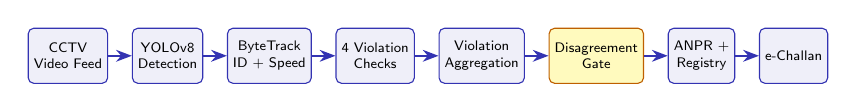
\begin{tikzpicture}[font=\tiny,
  b/.style={draw=dsblue,fill=dsblue!8,rounded corners=2pt,align=center,minimum height=7mm,inner sep=2pt},
  g/.style={draw=dOrange,fill=fYellow,rounded corners=2pt,align=center,minimum height=7mm,inner sep=2pt},
  a/.style={-{Stealth[length=2mm]},thick,dsblue}]
  \node[b] (c) {CCTV\\Video Feed};
  \node[b,right=3mm of c] (y) {YOLOv8\\Detection};
  \node[b,right=3mm of y] (t) {ByteTrack\\ID + Speed};
  \node[b,right=3mm of t] (v) {4 Violation\\Checks};
  \node[b,right=3mm of v] (ag) {Violation\\Aggregation};
  \node[g,right=3mm of ag] (gt) {Disagreement\\Gate};
  \node[b,right=3mm of gt] (an) {ANPR +\\Registry};
  \node[b,right=3mm of an] (ec) {e-Challan};
  \foreach \u/\w in {c/y,y/t,t/v,v/ag,ag/gt,gt/an,an/ec} \draw[a] (\u)--(\w);
\end{tikzpicture}
\end{frame}

%------------------------ LITERATURE REVIEW & SURVEY (3 BLOCKS) -------
\begin{frame}{LITERATURE REVIEW \& SURVEY}
\fontsize{6.4}{7.5}\selectfont
Published work divides into studies that perfect \textbf{one task in isolation} and \textbf{integrated systems} that
attempt several tasks at once, usually surrendering some precision in exchange.
\vspace{0.1em}
\begin{columns}[T,onlytextwidth]
\begin{column}{0.31\textwidth}
\begin{block}{1. Single-Task Detection Systems}
\begin{itemize}\setlength{\itemsep}{0.1em}
  \item Suman et al.\ [13]: 99.3\% mAP for helmet detection with YOLOv11
  \item Sutikno et al.\ [14]: 87--92\% on seat-belt compliance using YOLOv8 with CLAHE [19]
  \item Gautam and Kumar [15]: monocular speed error of roughly $\pm$2--3 km/h by pairing centroid tracking with
        Kalman smoothing
  \item Plate pipelines on YOLOv8 with EasyOCR [20] generally settle between 90\% and 94\% [3]
  \item Such scores come from curated datasets of clear views, whereas operational CCTV carries occlusion, oblique
        geometry, motion blur and low light.
\end{itemize}
\end{block}
\end{column}
\begin{column}{0.31\textwidth}
\begin{block}{2. Multi-Task and Integrated Systems}
\begin{itemize}\setlength{\itemsep}{0.1em}
  \item M.\,R.\ et al.\ [17]: 93--97\% on unified detection
  \item Kejriwal et al.\ [16]: 92.3\% mAP@0.5 for counting with YOLOv8 and DeepSORT
  \item Lin and Jhang [12]: 92.0\% at 37.9 FPS for flow monitoring by combining YOLOv5 with convolutional fuzzy
        neural networks
  \item Srinath et al.\ [4] couple vehicle recognition with e-challan generation
  \item Accident detection is usually posed standalone; Qamar et al.\ [18] report 96.76\% using CNN-based motion
        analysis
  \item Surveillance benchmarks such as UCF-Crime [23] show how hard crashes are to detect in low-resolution, distant CCTV.
\end{itemize}
\end{block}
\end{column}
\begin{column}{0.31\textwidth}
\begin{block}{3. Multi-Object Tracking}
\begin{itemize}\setlength{\itemsep}{0.1em}
  \item \textbf{SORT} [7]: Kalman filter and Hungarian assignment on IoU alone
  \item \textbf{DeepSORT} [5]: adds an appearance embedding, reducing identity switches through occlusion at the cost
        of a network evaluation per track per frame
  \item \textbf{ByteTrack} [6]: retains low-confidence boxes as second-stage association candidates; strong MOTA and
        IDF1 on MOT17 with no appearance model
  \item \textbf{Centroid} [2]: nearest-neighbour matching on box centres under a Euclidean gate --- cheapest
  \item Protocol: MOTA [8], IDF1 [9] and HOTA [10], as defined for the MOT benchmarks [11]
\end{itemize}
\end{block}
\end{column}
\end{columns}
\vspace{0.1em}
{\centering\tiny\itshape Every number here is quoted from the cited authors' publications; none is ours.\par}
\end{frame}

%------------------------ 2. PROBLEM STATEMENT ------------------------
\begin{frame}{2. PROBLEM STATEMENT}
\small
\begin{columns}[T,onlytextwidth]
\begin{column}{0.6\textwidth}
\hd{Five recurring deficiencies motivated this work:}
\scriptsize
\begin{itemize}\setlength{\itemsep}{0.2em}
\item \textbf{Violations are never correlated.} Three infringements by one vehicle ought to constitute one record
carrying three flags, not three unrelated entries.
\item \textbf{Databases are not live.} An officer downstream needs the violation within seconds, not the next morning.
\item \textbf{Challan generation stays manual.} Detection is automated, the paperwork is not, which reintroduces
precisely the bottleneck automation was meant to remove --- and when it is automated, a misread plate sends the notice
to the wrong citizen.
\item \textbf{Weather and incident monitoring are separate products.} Fog assessment and crash alerting run in their
own applications, despite fog being exactly the condition under which detection degrades and collisions become likelier.
\item \textbf{Model uncertainty is ignored.} If the network fires, the challan issues; no step defers a marginal
prediction to a person. An erroneous challan costs a citizen leave from work and a court appearance --- a heavy burden
to impose because a confidence score read 0.51 rather than 0.85.
\end{itemize}
\end{column}
\begin{column}{0.37\textwidth}
\vspace{0.2em}
\begin{beamercolorbox}[sep=0.5em,rounded=true]{block body}
\footnotesize\itshape
What is absent is a system that watches the feeds continuously and acts on what it sees.
\end{beamercolorbox}
\vspace{0.8em}
\centering
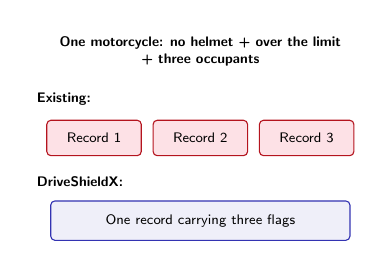
\begin{tikzpicture}[font=\tiny,
  r/.style={draw=dRed,fill=fRed,rounded corners=1.5pt,minimum width=12mm,minimum height=4.5mm,align=center},
  k/.style={draw=dsblue,fill=dsblue!8,rounded corners=1.5pt,minimum width=38mm,minimum height=5mm,align=center}]
  \node[font=\tiny\bfseries,align=center] (m) at (0,0) {One motorcycle: no helmet + over the limit\\+ three occupants};
  \node[font=\tiny\bfseries,anchor=west] at (-2.2,-0.6) {Existing:};
  \node[r] (r1) at (-1.35,-1.1) {Record 1};
  \node[r] (r2) at (0,-1.1) {Record 2};
  \node[r] (r3) at (1.35,-1.1) {Record 3};
  \node[font=\tiny\bfseries,anchor=west] at (-2.2,-1.65) {DriveShieldX:};
  \node[k] (k1) at (0,-2.15) {One record carrying three flags};
\end{tikzpicture}
\end{column}
\end{columns}
\end{frame}

%------------------------ 3. OBJECTIVES -------------------------------
\begin{frame}{3. OBJECTIVES}
\small
\vspace{0.3em}
\begin{enumerate}\setlength{\itemsep}{0.5em}
  \item To build \textbf{one pipeline} that recognises \textbf{four violation categories} from ordinary CCTV using
        \textbf{YOLOv8}.
  \item To hold a \textbf{single identity per vehicle} across frames --- by \textbf{ByteTrack}, with the centroid
        associator as the lightweight fallback --- so that multiple infringements resolve to one record.
  \item To recover plate numbers through a \textbf{two-stage ANPR} flow and \textbf{verify them against a registry}
        before an automated challan is composed.
  \item To interpose a \textbf{disagreement rule} that suspends issuance when the standalone and combined models
        conflict.
  \item To add \textbf{crash and fog monitoring} on the same feed.
  \item To evaluate all of it on documented data with \textbf{independent ground truth}, decomposed by ablation and
        reported with dispersion and significance where repeated observations exist --- and, where an evaluation could
        not be completed, to \textbf{say so explicitly} rather than to substitute an unsupported figure.
\end{enumerate}
\end{frame}

%------------------------ 4. RELATED WORK (1/2) -----------------------
\begin{frame}{4. RELATED WORK (1/2) -- DETECTION \& INTEGRATED SYSTEMS}
\scriptsize
\centering
\begin{tabularx}{\textwidth}{@{}L{0.2\textwidth}L{0.45\textwidth}Y@{}}
\toprule
\textbf{Work} & \textbf{Approach} & \textbf{Reported result}\\
\midrule
Suman et al.\ [13]      & Helmet detection with YOLOv11 & 99.3\% mAP\\
Sutikno et al.\ [14]    & Seat-belt compliance using YOLOv8 with CLAHE [19] & 87--92\%\\
Gautam and Kumar [15]   & Centroid tracking with Kalman smoothing, monocular speed & $\pm$2--3 km/h\\
Joshi et al.\ [3]       & Plate pipeline on YOLOv8 with EasyOCR [20] & 90--94\%\\
Srinath et al.\ [4]     & Vehicle recognition coupled with e-challan generation & --\\
M.\,R.\ et al.\ [17]    & Unified detection & 93--97\%\\
Kejriwal et al.\ [16]   & Counting with YOLOv8 and DeepSORT & 92.3\% mAP@0.5\\
Lin and Jhang [12]      & Flow monitoring, YOLOv5 with convolutional fuzzy neural networks & 92.0\% at 37.9 FPS\\
Qamar et al.\ [18]      & Accident detection, CNN-based motion analysis & 96.76\%\\
Sultani et al.\ [23]    & UCF-Crime: real-world surveillance video & crashes hard to detect in low-resolution, distant CCTV\\
\bottomrule
\end{tabularx}
\vspace{0.5em}

{\tiny\itshape Every number here is quoted from the cited authors' publications; none is ours. Such scores come from
curated datasets of clear views, whereas operational CCTV carries occlusion, oblique geometry, motion blur and low light.\par}
\end{frame}

%------------------------ 4. RELATED WORK (2/2) -----------------------
\begin{frame}{4. RELATED WORK (2/2) -- TRACKING \& COMPONENTS}
\scriptsize
\centering
\begin{tabularx}{\textwidth}{@{}L{0.33\textwidth}Y@{}}
\toprule
\textbf{Work} & \textbf{Role in DriveShieldX}\\
\midrule
Bewley et al.\ -- SORT [7]          & Kalman filter and Hungarian assignment on IoU alone\\
Wojke et al.\ -- DeepSORT [5]       & Appearance embedding; implemented as a comparison baseline\\
Zhang et al.\ -- ByteTrack [6]      & Low-confidence boxes as second-stage candidates; the \textbf{deployed tracker}\\
Dharmasaputra et al.\ [2]           & Centroid association; the \textbf{fallback}\\
Bernardin [8], Ristani [9], Luiten [10], Milan [11] & MOTA, IDF1, HOTA, MOT benchmarks; computed with the reference TrackEval implementation\\
Wen et al.\ -- UA-DETRAC [21]       & Ten sequences with published per-frame identity annotations (tracking ground truth)\\
Wilcoxon [22]                       & Signed-rank test, used where differences fail a Shapiro--Wilk check\\
Zuiderveld [19]; JaidedAI [20]; ankandrew [24] & CLAHE (seat belt); EasyOCR (fallback); fast-plate-ocr (plate recogniser)\\
Zenodo dataset [25]                 & Indian vehicles photographed by smartphone, with true plate strings (ANPR)\\
Tran et al.\ [27]; Kay et al.\ [28] & R3D-18 pretrained on Kinetics-400 (crash model)\\
He et al.\ [29]                     & Dark-channel prior (fog index)\\
Motor Vehicles (Amendment) Act 2019 [26] & Statutory penalties applied by the e-Challan engine\\
\bottomrule
\end{tabularx}
\end{frame}

%------------------------ 5. RESEARCH GAPS ----------------------------
\begin{frame}{5. RESEARCH GAPS}
\small
\centering
\begin{tabularx}{0.94\textwidth}{@{}L{0.25\textwidth}Y@{}}
\toprule
\textbf{Area} & \textbf{Identified Gap}\\
\midrule
Violation correlation   & No work surveyed correlates several infractions to one vehicle identity.\\
Enforcement chain       & None carries detection through ANPR and a registry check to challan issuance without a manual step.\\
Weather \& collision    & Weather and collision analysis are published as standalone systems although they consume the identical feed.\\
Model uncertainty       & No pipeline interposes a state in which a low-confidence prediction is deferred to a person rather than acted upon.\\
\midrule
Tracking in dense scenes& Centroid association is cheapest and widely used in traffic work [2], yet its behaviour in dense scenes is rarely quantified against stronger trackers.\\
\bottomrule
\end{tabularx}
\vspace{0.6em}

{\color{dsblue}\textbf{The deficiencies enumerated in the introduction recur throughout this literature.
DriveShieldX addresses all four.}}
\end{frame}

%------------------------ 6. PROPOSED SYSTEM -- ARCHITECTURE ----------
\begin{frame}[t]{6. PROPOSED SYSTEM -- SYSTEM ARCHITECTURE}
\vspace{-0.35em}
\centering
\resizebox{0.93\textwidth}{!}{%
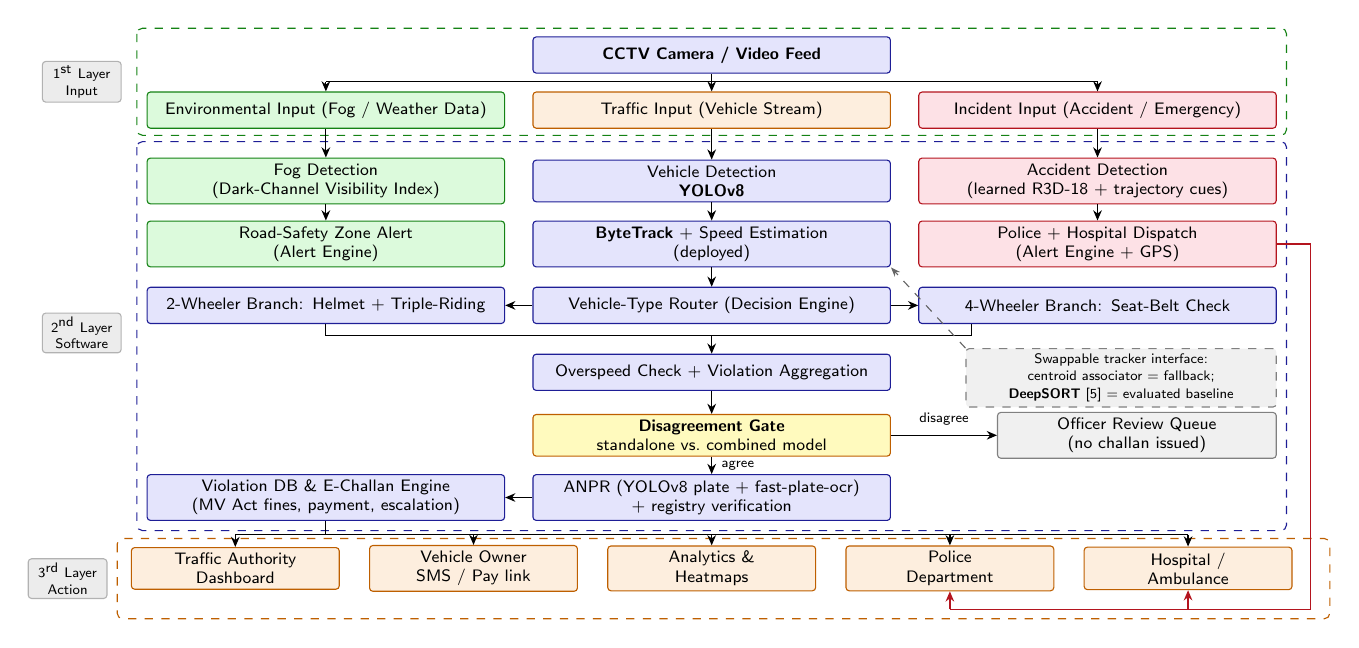
\begin{tikzpicture}[x=1mm,y=1mm,font=\fontsize{6}{6.9}\selectfont,
  bx/.style={draw,rounded corners=1.2pt,align=center,text width=44mm,minimum height=4.6mm,inner sep=0.7mm,line width=0.4pt},
  gB/.style={bx,draw=dGreen,fill=fGreen},
  oB/.style={bx,draw=dOrange,fill=fOrange},
  rB/.style={bx,draw=dRed,fill=fRed},
  bB/.style={bx,draw=dBlue,fill=fBlue},
  yB/.style={bx,draw=dOrange,fill=fYellow},
  aB/.style={bx,draw=dOrange,fill=fOrange,text width=25mm},
  tag/.style={draw=gray!60,fill=gray!15,rounded corners=1.2pt,align=center,text width=9mm,inner sep=0.5mm,font=\fontsize{5.2}{6}\selectfont},
  ar/.style={-{Stealth[length=1.3mm,width=1.1mm]},line width=0.45pt},
  ln/.style={line width=0.45pt},
  lb/.style={font=\fontsize{4.8}{5}\selectfont}]
\def\E{36}\def\T{85}\def\I{134}
\node[bB,font=\fontsize{6}{6.9}\selectfont\bfseries] (cctv) at (\T,0) {CCTV Camera / Video Feed};
\node[gB] (env) at (\E,-7) {Environmental Input (Fog / Weather Data)};
\node[oB] (tin) at (\T,-7) {Traffic Input (Vehicle Stream)};
\node[rB] (iin) at (\I,-7) {Incident Input (Accident / Emergency)};
\node[gB] (fog)  at (\E,-16) {Fog Detection\\(Dark-Channel Visibility Index)};
\node[bB] (vdet) at (\T,-16) {Vehicle Detection\\\textbf{YOLOv8}};
\node[rB] (acc)  at (\I,-16) {Accident Detection\\(learned R3D-18 + trajectory cues)};
\node[gB] (zone) at (\E,-24) {Road-Safety Zone Alert\\(Alert Engine)};
\node[bB] (trk)  at (\T,-24) {\textbf{ByteTrack} + Speed Estimation\\(deployed)};
\node[rB] (disp) at (\I,-24) {Police + Hospital Dispatch\\(Alert Engine + GPS)};
\node[bB] (tw)   at (\E,-31.8) {2-Wheeler Branch: Helmet + Triple-Riding};
\node[bB] (rtr)  at (\T,-31.8) {Vehicle-Type Router (Decision Engine)};
\node[bB] (fw)   at (\I,-31.8) {4-Wheeler Branch: Seat-Belt Check};
\node[bB] (agg)  at (\T,-40.3) {Overspeed Check + Violation Aggregation};
\node[bx,draw=gray,dashed,fill=fGray,text width=38mm,font=\fontsize{5.4}{6.2}\selectfont] (note) at (\I+3,-41.0) {Swappable tracker interface:\\centroid associator = fallback;\\\textbf{DeepSORT} [5] = evaluated baseline};
\node[yB] (gate) at (\T,-48.3) {\textbf{Disagreement Gate}\\standalone vs.\ combined model};
\node[bx,draw=gray,fill=fGray,text width=34mm] (rev) at (\I+5,-48.3) {Officer Review Queue\\(no challan issued)};
\node[bB] (anpr) at (\T,-56.2) {ANPR (YOLOv8 plate + fast-plate-ocr)\\+ registry verification};
\node[bB] (db)   at (\E,-56.2) {Violation DB \& E-Challan Engine\\(MV Act fines, payment, escalation)};
\node[aB] (a1) at (24.5,-65.2)  {Traffic Authority\\Dashboard};
\node[aB] (a2) at (54.75,-65.2) {Vehicle Owner\\SMS / Pay link};
\node[aB] (a3) at (85,-65.2)    {Analytics \&\\Heatmaps};
\node[aB] (a4) at (115.25,-65.2){Police\\Department};
\node[aB] (a5) at (145.5,-65.2) {Hospital /\\Ambulance};
\begin{scope}[on background layer]
 \draw[dGreen,dashed,rounded corners=2pt] (12,3.4) rectangle (158,-10.2);
 \draw[dBlue,dashed,rounded corners=2pt] (12,-11.0) rectangle (158,-60.4);
 \draw[dOrange,dashed,rounded corners=2pt] (9.5,-61.4) rectangle (163.5,-71.6);
\end{scope}
\node[tag] at (5,-3.4)  {1\textsuperscript{st} Layer\\Input};
\node[tag] at (5,-35.3) {2\textsuperscript{nd} Layer\\Software};
\node[tag] at (3.2,-66.5) {3\textsuperscript{rd} Layer\\Action};
\draw[ln] (cctv.south) -- (\T,-3.4);
\draw[ln] (\E,-3.4) -- (\I,-3.4);
\foreach \n/\x in {env/\E,tin/\T,iin/\I} \draw[ar] (\x,-3.4) -- (\n.north);
\draw[ar] (env) -- (fog);  \draw[ar] (tin) -- (vdet); \draw[ar] (iin) -- (acc);
\draw[ar] (fog) -- (zone); \draw[ar] (vdet) -- (trk); \draw[ar] (acc) -- (disp);
\draw[ar] (trk) -- (rtr);
\draw[ar] (rtr) -- (tw);   \draw[ar] (rtr) -- (fw);
\draw[ln] (tw.south) -- (\E,-35.6) -- (\I-16,-35.6) -- (\I-16,-34.1);
\draw[ar] (\T,-35.6) -- (agg.north);
\draw[ar] (agg) -- (gate);
\draw[ar] (gate) -- node[above,lb]{disagree} (rev);
\draw[ar] (gate) -- node[right,lb]{agree} (anpr);
\draw[ar] (anpr) -- (db);
\draw[-{Stealth[length=1.2mm]},dashed,gray!80!black,line width=0.4pt] (note.north west) -- (trk.south east);
\draw[ln] (db.south) -- (\E,-60.9);
\draw[ln] (24.5,-60.9) -- (145.5,-60.9);
\foreach \n/\x in {a1/24.5,a2/54.75,a3/85,a4/115.25,a5/145.5} \draw[ar] (\x,-60.9) -- (\n.north);
\draw[ln,dRed] (disp.east) -- (161,-24) -- (161,-70.4) -- (115.25,-70.4);
\draw[ar,dRed] (115.25,-70.4) -- (a4.south);
\draw[ar,dRed] (145.5,-70.4) -- (a5.south);
\end{tikzpicture}
}

\vspace{0.1em}
{\centering\tiny Fig.~1: DriveShieldX system architecture. The deployed configuration tracks with ByteTrack; the centroid
associator is the fallback at the same interface and DeepSORT is implemented as an evaluated baseline. The disagreement
gate is the single point at which an automatic challan can be suppressed in favour of human review, and only a
registry-verified plate leads to an automatic challan.\par}
\end{frame}

%------------------------ 6. PROPOSED SYSTEM -- VIOLATION MODULES -----
\begin{frame}{6. PROPOSED SYSTEM -- VIOLATION MODULES}
\scriptsize
Vehicle class --- two-wheeler or four-wheeler --- selects the violation branch that executes next.
\vspace{0.4em}
\begin{columns}[T,onlytextwidth]
\begin{column}{0.32\textwidth}
\begin{block}{Two-Wheeler Branch}
\textbf{Helmet.} A YOLOv8 model trained on \texttt{helmet}/\texttt{no\_helmet} instances evaluates the rider head
region inside each detected motorcycle box; absence raises a \texttt{no\_helmet} event.\\[0.4em]
\textbf{Triple-riding.} Person detections whose boxes intersect a two-wheeler box above an overlap threshold are
counted, and a count exceeding two logs a \texttt{three\_seater} event against that track.
\end{block}
\end{column}
\begin{column}{0.32\textwidth}
\begin{block}{Four-Wheeler Branch}
\textbf{Seat belt.} The occupant associated with a car is cropped and classified for belt presence, with CLAHE [19]
applied beforehand to recover contrast under low light and glare. Because occupants behind glass are often missed by
the person detector, a car with no associated person is now checked on its windscreen band and on its driver and
passenger halves instead of being skipped; a violation still requires the no-belt score to beat the belt score by a
margin.
\end{block}
\end{column}
\begin{column}{0.32\textwidth}
\begin{block}{Every Track}
\textbf{Over-speed.} The speed of Equation~(1) is compared against a per-camera, per-zone limit and graded into low,
medium, high and extreme bands.\\[0.4em]
\textbf{Aggregation and the disagreement gate.} All flags active for a track are merged before ANPR is invoked, so one
challan carries every concurrent infraction. Immediately before issuance the gate compares the standalone helmet
classifier against the combined multi-class detector on the same crop.
\end{block}
\end{column}
\end{columns}
\vspace{0.4em}
With $p_s$ and $p_c$ their positive-class confidences and $\theta$ the issuance threshold, a challan is composed
automatically only if both exceed $\theta$ or both fall below it; otherwise the event is written to the officer review
queue with its evidence crop and no notice is dispatched.
\end{frame}

%------------------------ 6. PROPOSED SYSTEM -- ACCIDENT & FOG --------
\begin{frame}{6. PROPOSED SYSTEM -- ACCIDENT \& FOG MONITORING}
\scriptsize
\begin{columns}[T,onlytextwidth]
\begin{column}{0.56\textwidth}
\hd{\small Accidents}
\begin{itemize}\setlength{\itemsep}{0.2em}
  \item The first accident detector was rule-based: it flagged abrupt stops, reversals and sudden box overlap between
        tracked vehicles. It found almost no crashes on low-resolution CCTV, because the tracks it relies on fragment
        exactly at the moment of impact. It is now a fallback.
  \item The deployed detector is a video model that looks at the whole picture: frames are resampled to 8 FPS and
        resized to $128\times171$, and each 2-second window of 16 frames, centre-cropped to $112\times112$, is
        classified as crash or no crash by \textbf{R3D-18} [27] pretrained on Kinetics-400 [28] and fine-tuned on
        hand-labelled crash windows.
  \item An alert is raised when the crash probability exceeds the validation-chosen threshold for two consecutive
        windows; it is then suppressed for 60 s.
  \item A confirmed alert is stored with its snapshot and sent to the control room together with the nearest police
        station and hospital, located from the camera's GPS position and OpenStreetMap data, with distance and map links.
\end{itemize}
\end{column}
\begin{column}{0.4\textwidth}
\hd{\small Fog}
\begin{itemize}\setlength{\itemsep}{0.2em}
  \item A visibility index combines the \textbf{dark-channel prior} [29], image contrast and edge density on the road
        region of each frame into a fog score between 0 and 1.
  \item Graded into clear, light haze, moderate fog and dense fog.
  \item A camera's own clear-weather baseline, when available, makes the score relative.
  \item A sustained moderate or dense grade raises a zone advisory.
\end{itemize}
\vspace{0.4em}
\centering
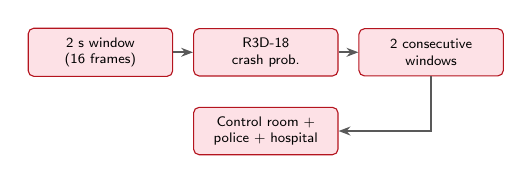
\begin{tikzpicture}[font=\tiny,
  b/.style={draw=dRed,fill=fRed,rounded corners=2pt,align=center,minimum height=6mm,text width=16mm},
  a/.style={-{Stealth[length=1.5mm]},thick,gray!70!black}]
  \node[b] (a) at (0,0) {2 s window\\(16 frames)};
  \node[b] (b) at (2.1,0) {R3D-18\\crash prob.};
  \node[b] (c) at (4.2,0) {2 consecutive\\windows};
  \node[b] (d) at (2.1,-1.0) {Control room +\\police + hospital};
  \draw[a] (a)--(b); \draw[a] (b)--(c); \draw[a] (c) |- (d);
\end{tikzpicture}
\end{column}
\end{columns}
\end{frame}

%------------------------ 7. METHODOLOGY ------------------------------
\begin{frame}{7. RESEARCH METHODOLOGY -- SYSTEM ARCHITECTURE AND DATA FLOW}
\scriptsize
\centering
\begin{tabularx}{\textwidth}{@{}c L{0.19\textwidth} Y@{}}
\toprule
\textbf{Step} & \textbf{Stage} & \textbf{Processing}\\
\midrule
1 & Input              & Raw frames enter pre-processing.\\
2 & Object detection   & YOLOv8 [1]: each frame passes through the network once, yielding boxes, class labels and
                         confidences. Five weight sets are loaded concurrently --- \texttt{person}, \texttt{twowheeler},
                         \texttt{helmet}, \texttt{seatbelt} and \texttt{plate}.\\
3 & Tracking           & ByteTrack associates detections across frames and supplies the persistent identity on which
                         violation aggregation depends; the centroid associator is the fallback.\\
4 & Speed estimation   & Centroid displacement, frame rate, and a pixel-to-real-world calibration factor [15] (Eq.~1);
                         any reading above 200 km/h is marked disputed and sent to an officer.\\
5 & Vehicle-type routing & Vehicle class --- two-wheeler or four-wheeler --- selects the violation branch that executes next.\\
6 & Aggregation \& gate & All raised flags are collected; the disagreement gate issues or defers to officer review.\\
7 & ANPR \& registry   & YOLOv8 localises the plate; the padded crop is read by fast-plate-ocr [24] (EasyOCR [20]
                         fallback); Indian plate grammar repairs look-alike glyphs; the plate is verified against the
                         vehicle registry.\\
8 & e-Challan          & The completed record is written to the Violation Database, from which the e-Challan engine
                         notifies the registered owner and the Traffic Authority.\\
\bottomrule
\end{tabularx}
\vspace{0.4em}

{\color{dsblue}\textbf{Fog assessment and accident detection consume the same frames on separate threads and so do not
extend the latency of the primary path.}}
\end{frame}

%------------------------ 7(a). DFD LEVEL 2 -- SPEED DETECTION --------
\begin{frame}[t]{7(a). DFD LEVEL 2 -- CAMERA $\rightarrow$ FRAME $\rightarrow$ SPEED DETECTION}
\vspace{-0.3em}
\centering
\resizebox{0.95\textwidth}{!}{%
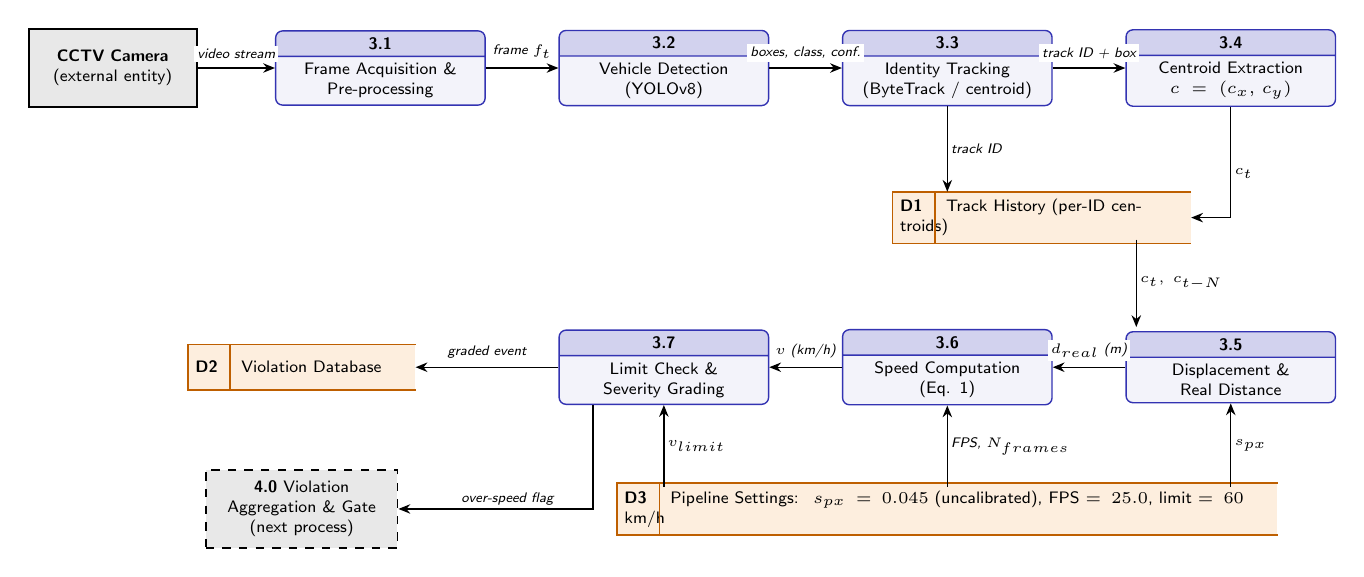
\begin{tikzpicture}[x=1mm,y=1mm,font=\fontsize{6.2}{7.2}\selectfont,
  proc/.style={rectangle split,rectangle split parts=2,draw=dsblue,rounded corners=2.5pt,
               align=center,text width=25mm,inner sep=0.8mm,line width=0.5pt,
               rectangle split part fill={dsblue!22,dsblue!6}},
  ent/.style={draw=black,fill=gray!18,align=center,text width=19mm,minimum height=10mm,line width=0.7pt},
  st/.style={align=left,minimum height=5.6mm,inner sep=0.9mm,fill=fOrange},
  fl/.style={-{Stealth[length=1.5mm,width=1.2mm]},line width=0.5pt},
  lab/.style={font=\fontsize{5.3}{6}\selectfont\itshape,fill=white,inner sep=0.4mm}]
% ---- external entity
\node[ent] (cam) at (0,0) {\textbf{CCTV Camera}\\(external entity)};
% ---- row 1
\node[proc] (p1) at (34,0)  {\textbf{3.1}\nodepart{two}Frame Acquisition \&\\Pre-processing};
\node[proc] (p2) at (70,0)  {\textbf{3.2}\nodepart{two}Vehicle Detection\\(YOLOv8)};
\node[proc] (p3) at (106,0) {\textbf{3.3}\nodepart{two}Identity Tracking\\(ByteTrack / centroid)};
\node[proc] (p4) at (142,0) {\textbf{3.4}\nodepart{two}Centroid Extraction\\$c=(c_x,\,c_y)$};
% ---- data store D1
\dstore{d1}{118,-19}{\textbf{D1}\hspace{3mm}Track History (per-ID centroids)}{36mm}
% ---- row 3 (right to left)
\node[proc] (p5) at (142,-38) {\textbf{3.5}\nodepart{two}Displacement \&\\Real Distance};
\node[proc] (p6) at (106,-38) {\textbf{3.6}\nodepart{two}Speed Computation\\(Eq. 1)};
\node[proc] (p7) at (70,-38)  {\textbf{3.7}\nodepart{two}Limit Check \&\\Severity Grading};
\dstore{d2}{24,-38}{\textbf{D2}\hspace{3mm}Violation Database}{27mm}
% ---- settings store + next process
\dstore{d3}{106,-56}{\textbf{D3}\hspace{3mm}Pipeline Settings: \ $s_{px}=0.045$ (uncalibrated),\ FPS $=25.0$,\ limit $=60$ km/h}{82mm}
\node[ent,dashed,text width=22mm] (p8) at (24,-56) {\textbf{4.0} Violation\\Aggregation \& Gate\\(next process)};
% ---- flows
\draw[fl] (cam) -- node[lab,above=0.7mm]{video stream} (p1);
\draw[fl] (p1) -- node[lab,above=0.7mm]{frame $f_t$} (p2);
\draw[fl] (p2) -- node[lab,above=0.7mm]{boxes, class, conf.} (p3);
\draw[fl] (p3) -- node[lab,above=0.7mm]{track ID + box} (p4);
\draw[fl] (p3.south) -- node[lab,right]{track ID} (p3.south |- d1.north);
\draw[fl] (p4.south) |- node[lab,pos=0.3,right]{$c_t$} (d1.east);
\draw[fl] (130,-21.8) -- node[lab,right]{$c_t,\ c_{t-N}$} (130,-32.9);
\draw[fl] (p5) -- node[lab,above=0.7mm]{$d_{real}$ (m)} (p6);
\draw[fl] (p6) -- node[lab,above=0.7mm]{$v$ (km/h)} (p7);
\draw[fl] (p7) -- node[lab,above=0.7mm]{graded event} (d2);
\draw[fl] (142,-53.2) -- node[lab,right]{$s_{px}$} (p5.south);
\draw[fl] (106,-53.2) -- node[lab,right]{FPS, $N_{frames}$} (p6.south);
\draw[fl] (70,-53.2) -- node[lab,right]{$v_{limit}$} (p7.south);
\draw[fl] ([xshift=-9mm]p7.south) |- node[lab,pos=0.72,above]{over-speed flag} (p8.east);
\end{tikzpicture}}

\vspace{0.3em}
{\scriptsize \hd{Legend:} rounded box = process \quad open box = data store \quad grey box = external entity \quad
arrow = data flow\\[0.25em]
\hd{Level-2 expansion of Process 3.0 (Speed Detection)} \quad | \quad \hd{Eq. 1:} \ $v=\dfrac{d_{real}\times \text{FPS}}{N_{frames}}\times 3.6$ km/h,
\quad $d_{real}=s_{px}\cdot\lVert c_t-c_{t-N}\rVert_2$\par}
\end{frame}


%------------------------ 8. SYSTEM IMPLEMENTATION --------------------
\begin{frame}{8. SYSTEM IMPLEMENTATION}
\begin{columns}[T,onlytextwidth]
\begin{column}{0.42\textwidth}
\scriptsize
\hd{\footnotesize A. Frontend} (Streamlit interface)
\begin{itemize}\setlength{\itemsep}{0.05em}
  \item Traffic Authority Dashboard
  \item Officer Review Queue (no challan issued)
  \item Analytics \& Heatmaps
  \item Vehicle Owner: SMS / Pay link
\end{itemize}
\vspace{0.3em}
\hd{\footnotesize B. Backend Processing}
\begin{itemize}\setlength{\itemsep}{0.05em}
  \item Five weight sets are loaded concurrently
  \item ByteTrack, invoked through the Ultralytics interface; centroid associator as fallback
  \item Fog assessment and accident detection consume the same frames on separate threads
  \item Inference runs on a CPU (PyTorch 2.13.0+cpu) with SQLite storage and a Streamlit interface
\end{itemize}
\vspace{0.2em}
{\scriptsize\color{dsblue}\textbf{Frame $\rightarrow$ YOLOv8 $\rightarrow$ ByteTrack $\rightarrow$ Router $\rightarrow$ Branch
$\rightarrow$ Gate $\rightarrow$ ANPR $\rightarrow$ Registry $\rightarrow$ DB $\rightarrow$ e-Challan}}
\end{column}
\begin{column}{0.55\textwidth}
\hd{\small Technology Stack}\\[0.2em]
\scriptsize
\begin{tabularx}{\linewidth}{@{}L{0.3\linewidth}Y@{}}
\toprule
\textbf{Component} & \textbf{Technology / Approach}\\
\midrule
Detection framework  & Ultralytics 8.4.121 (helmet, seat belt) and 8.4.60 (two-wheeler, plate), YOLOv8 [1]\\
Detectors            & YOLOv8s (helmet, seat belt); YOLOv8n (two-wheeler, plate); YOLO11n (person, COCO, unmodified)\\
Tracking             & ByteTrack [6] (deployed); centroid (fallback); DeepSORT [5] (evaluated baseline)\\
Plate reading        & fast-plate-ocr [24]; EasyOCR [20] fallback\\
Crash model          & R3D-18 [27] pretrained on Kinetics-400 [28]; fine-tuned on a free cloud GPU (T4)\\
Fog index            & Dark-channel prior [29], image contrast and edge density\\
Pre-processing       & CLAHE [19] (seat belt); padded plate crop\\
Inference runtime    & PyTorch 2.13.0+cpu, on a CPU\\
Database / UI        & SQLite / Streamlit\\
Payment / SMS        & Razorpay test gateway / Android SMS gateway\\
\bottomrule
\end{tabularx}
\end{column}
\end{columns}
\end{frame}

%------------------------ 8. EXPERIMENTAL SETUP -- MODELS -------------
\begin{frame}{8. EXPERIMENTAL SETUP -- MODELS AND TRAINING PROVENANCE}
\scriptsize
Five detectors run concurrently in deployment. Four were fine-tuned for this work; the person detector is used
unmodified from COCO pre-training. Table~1 records what each was trained from and on, recovered from the training
arguments Ultralytics embeds inside every checkpoint.
\vspace{0.5em}

\centering
{\tiny Table 1: Model provenance, recovered from the \texttt{train\_args} block of each checkpoint.}\\[0.2em]
\begin{tabular}{@{}llp{42mm}ccc@{}}
\toprule
\textbf{Detector} & \textbf{Backbone} & \textbf{Classes} & \textbf{Epochs} & \textbf{Batch} & \textbf{Seed}\\
\midrule
Helmet & YOLOv8s & helmet, no\_helmet & 100 & 16 & 42\\
Seat belt & YOLOv8s & seatbelt, no\_seatbelt & 100 & 16 & 42\\
Two-wheeler & YOLOv8n & with\_helmet, without\_helmet, triple\_riding & 100 & 32 & 0\\
Plate & YOLOv8n & License\_Plate & 80 & 32 & 0\\
Person & YOLO11n & COCO, unmodified & -- & -- & --\\
Crash model & R3D-18 & crash, no crash & 10 (best 5) & 16 & 0\\
\bottomrule
\end{tabular}
\vspace{0.6em}

\raggedright
\textbf{A disclosure about the detector training corpora.} The four detector fine-tuning datasets were assembled and
trained in a hosted notebook environment, and their composition survives in the checkpoints only as notebook-local
paths. Those directories are not presently in our possession, so neither per-split image counts nor per-class
instance counts can be stated, and an earlier draft's figure of 727 validation images is withdrawn. Recovering the
corpora and re-running per-class validation is listed as future work.
\end{frame}

%------------------------ 8. EXPERIMENTAL SETUP -- DATA ---------------
\begin{frame}{8. EXPERIMENTAL SETUP -- EVALUATION DATA}
\scriptsize
Every evaluation uses ground truth that is independent of the system being scored: published annotations, a dataset's
own labels, or labels written by the authors on held-out material that the models never saw.
\begin{itemize}\setlength{\itemsep}{0.25em}
\item \textbf{Tracking:} ten UA-DETRAC [21] sequences (MVI\_20012, 20065, 39761, 40152, 40212, 40742, 40775, 40891,
40992, 63563) with published per-frame identity annotations.
\item \textbf{Disagreement gate:} 1204 two-wheeler rider crops sampled from five project videos; the 286 events that
an OR rule would have fined were each judged by the authors from the crop alone, with the model scores hidden
(\emph{violation}, \emph{no violation} or \emph{unclear}).
\item \textbf{ANPR:} the public Number Plate Identification dataset [25] of Indian vehicles photographed by
smartphone, whose authors supply the true plate strings. 300 photos were used for error analysis and development; a
disjoint set of 291 photos was held out and scored once.
\item \textbf{Accidents:} UCF-Crime [23], real CCTV. The test set is all 23 RoadAccidents videos with published
frame-level crash timings plus 23 normal videos (0.51 h after trimming to the crash window $\pm$30 s and the first
60 s of each normal video). Training used the other 127 RoadAccidents videos, whose crash start and end times the
authors marked by hand, and 100 further normal videos; none overlaps the test set.
\item \textbf{Fog:} 10 foggy and 10 clear daytime road clips from different cameras (free stock footage), plus a
controlled test in which synthetic haze following the atmospheric scattering model is added to 100 real frames.
\item \textbf{Throughput:} five project clips (two-wheeler traffic, in-cabin seat-belt material and 1080p road
traffic), 200 frames each.
\end{itemize}
\end{frame}

%------------------------ 8. EXPERIMENTAL SETUP -- TRAINING -----------
\begin{frame}{8. EXPERIMENTAL SETUP -- TRAINING, SETTINGS AND STATISTICS}
\scriptsize
\begin{columns}[T,onlytextwidth]
\begin{column}{0.49\textwidth}
\hd{\small Detectors}
\begin{itemize}\setlength{\itemsep}{0.15em}
  \item Ultralytics 8.4.121 (helmet, seat belt) and 8.4.60 (two-wheeler, plate) from COCO-pretrained weights at
        $640\times640$ input with Ultralytics' default augmentation and its automatic optimiser choice; each model
        was trained once.
\end{itemize}
\hd{\small Crash model (free cloud GPU, T4)}
\begin{itemize}\setlength{\itemsep}{0.15em}
  \item Windows labelled crash when their centre lies between 0.5 s before the marked start and 1 s after the marked
        end; no-crash when they lie at least 3 s away from any crash or come from a normal video; ambiguous windows are not used.
  \item 2706 crash and 24\,844 no-crash windows; classes balanced in every epoch (3000 windows), random crops,
        horizontal flips and brightness jitter; AdamW at $10^{-4}$ (head $10^{-3}$) with cosine decay.
  \item A validation split of 45 training videos, divided by video, selected the epoch and the alarm threshold; the
        test set played no part in either choice.
\end{itemize}
\end{column}
\begin{column}{0.48\textwidth}
\hd{\small Pipeline settings}
\begin{itemize}\setlength{\itemsep}{0.15em}
  \item Pixel-to-metre scale 0.045 (uncalibrated, one constant for all cameras)
  \item Assumed source frame rate 25.0 FPS; speed limit 60 km/h; plausibility hold above 200 km/h
  \item Seat-belt confirmation over 3 observations at a 0.12 margin
  \item Disagreement-gate threshold $\theta = 0.15$
\end{itemize}
\hd{\small Statistical protocol}
\begin{itemize}\setlength{\itemsep}{0.15em}
  \item Tracker comparisons are paired by sequence, each tracker consuming an identical cached detection stream, so
        any difference is attributable to association alone.
  \item Two-sided paired $t$-test where the differences pass a Shapiro--Wilk check and the Wilcoxon signed-rank test
        [22] otherwise, with Holm--Bonferroni correction and exact $p$-values reported.
  \item Each detector was trained once, so no dispersion is reported for detection metrics.
\end{itemize}
\end{column}
\end{columns}
\end{frame}

%------------------------ 9. ALGORITHMS -------------------------------
\begin{frame}{9. ALGORITHMS}
\begin{columns}[T,onlytextwidth]
\begin{column}{0.46\textwidth}
\hd{\small Algorithm 1: Centroid Association (fallback) \& Speed}\\
{\tiny\textit{Input:} detections of frame $t$, $\tau_d$, $\tau_a$, $s_{px}$, FPS \ \ \textit{Output:} track IDs, speed $v$}
\scriptsize
\begin{enumerate}\setlength{\itemsep}{0em}
  \item For each box, take the midpoint $(c_x, c_y)$.
  \item Match centroids in consecutive frames by minimum Euclidean distance.
  \item Accept a match only within the gating radius $\tau_d$.
  \item Matched: keep the identifier; append to the displacement history.
  \item Unmatched detection: new identifier.
  \item Unmatched track: retain for $\tau_a$ frames before deletion, so that short detection dropouts are absorbed.
  \item $d_{real} = s_{px}\cdot\lVert c_t - c_{t-N}\rVert_2$.
  \item Speed $v$ by Eq.~1 (km/h).
  \item Above 200 km/h: marked disputed and sent to an officer.
  \item Otherwise compare with the per-camera, per-zone limit; grade low / medium / high / extreme.
\end{enumerate}
\end{column}
\begin{column}{0.51\textwidth}
\hd{\small Algorithm 2: Multi-Violation Detection \& e-Challan}\\
{\tiny\textit{Input:} CCTV video stream \ \ \textit{Output:} e-challan or officer-review entry}
\scriptsize
\begin{enumerate}\setlength{\itemsep}{0em}
  \item Raw frames enter pre-processing.
  \item YOLOv8 once per frame (five weight sets).
  \item Track with ByteTrack (Algorithm 1 as fallback); estimate speed.
  \item Route by vehicle class (two-wheeler / four-wheeler).
  \item Two-wheeler: helmet on the rider head region $\rightarrow$ \texttt{no\_helmet}; persons over the overlap
        threshold, count $>2$ $\rightarrow$ \texttt{three\_seater}.
  \item Four-wheeler: CLAHE; occupant crop, or windscreen band and driver and passenger halves $\rightarrow$ belt
        presence.
  \item Over-speed check against the zone limit.
  \item Merge all flags active for the track.
  \item Gate: both $p_s,p_c>\theta$ or both $<\theta$ $\rightarrow$ continue; otherwise officer review queue, no notice.
  \item ANPR: YOLOv8 plate $\rightarrow$ padded crop $\rightarrow$ fast-plate-ocr; Indian plate grammar.
  \item Valid registration found in the registry $\rightarrow$ automatic challan; otherwise officer, reason recorded.
  \item MV Act penalty or graduated schedule, whichever is higher; SMS with a payment link.
\end{enumerate}
\end{column}
\end{columns}
\end{frame}

%------------------------ 9. ALGORITHM FORMULATION --------------------
\begin{frame}{9. ALGORITHM -- MATHEMATICAL FORMULATION}
\begin{columns}[T,onlytextwidth]
\begin{column}{0.49\textwidth}
\hd{\small Tracking \& Speed}
\footnotesize
\begin{itemize}\setlength{\itemsep}{0.25em}
  \item Centroid of box $(x_1,y_1,x_2,y_2)$:\;
        $c=(c_x,c_y)=\left(\frac{x_1+x_2}{2},\frac{y_1+y_2}{2}\right)$
  \item Association: $j^{*}=\arg\min_j \lVert c_i^{\,t}-c_j^{\,t-1}\rVert_2$, \ accepted iff
        $\lVert c_i^{\,t}-c_{j^*}^{\,t-1}\rVert_2\le\tau_d$
  \item Equation (1):
        \[\begin{aligned}v &= \frac{d_{\mathrm{real}}\times \mathrm{FPS}}{N_{\mathrm{frames}}}\times 3.6 \quad (\mathrm{km/h}),\\
          d_{\mathrm{real}} &= s_{px}\cdot \lVert \mathbf{c}_t-\mathbf{c}_{t-N}\rVert_2\end{aligned}\]
  \item $s_{px}$ is a pixel-to-metre scale and $N_{\mathrm{frames}}$ the frames elapsed between reference lines.
  \item $s_{px}$ is presently a single uncalibrated constant of 0.045 shared by every camera, and the frame rate
        substituted for FPS is fixed at 25.0 rather than read from the clip.
\end{itemize}
\end{column}
\begin{column}{0.49\textwidth}
\hd{\small Violation Rules, Gate \& Alerts}
\footnotesize
\begin{itemize}\setlength{\itemsep}{0.25em}
  \item Over-speed: $v$ compared against a per-camera, per-zone limit (60 km/h)
  \item Triple-riding: \ $n=\sum_k \mathbf{1}\!\left[\text{overlap}(P_k,B_{2W})>\tau_o\right]$;
        \ \texttt{three\_seater} if $n>2$
  \item Disagreement gate ($p_s$, $p_c$ = positive-class confidences, $\theta$ = issuance threshold $=0.15$):
        \[\text{Issue}\iff (p_s>\theta \wedge p_c>\theta)\ \vee\ (p_s<\theta \wedge p_c<\theta)\]
        otherwise $\rightarrow$ officer review queue, no notice dispatched
  \item Crash alert: crash probability above the validation-chosen threshold for two consecutive windows; then
        suppressed for 60 s
  \item Fog: score between 0 and 1 $\rightarrow$ clear, light haze, moderate fog, dense fog
\end{itemize}
\end{column}
\end{columns}
\end{frame}

%------------------------ 10. FUNCTIONAL MODULES ----------------------
\begin{frame}{10. FUNCTIONAL MODULES}
\scriptsize
\renewcommand{\arraystretch}{1.05}
\centering
\begin{tabularx}{\textwidth}{@{}L{0.24\textwidth}L{0.33\textwidth}Y@{}}
\toprule
\textbf{Module} & \textbf{Input} & \textbf{Output}\\
\midrule
Object Detection (YOLOv8)       & Video frame                                & Boxes, class labels, confidences\\
Tracking (ByteTrack / centroid) & Per-frame detections                       & Persistent vehicle identity + displacement history\\
Speed Estimation                & Displacement history, FPS, $s_{px}$        & Speed $v$ (km/h); above 200 km/h held for an officer\\
Vehicle-Type Router             & Vehicle class                              & Two-wheeler or four-wheeler branch\\
Helmet Detection                & Rider head region inside motorcycle box    & \texttt{no\_helmet} event\\
Triple-Riding Detection         & Person boxes + two-wheeler box             & \texttt{three\_seater} event (count $>2$)\\
Seat-Belt Detection             & Occupant crop or windscreen band (CLAHE)   & Seat-belt violation\\
Over-speed Check                & Speed + per-camera, per-zone limit         & Low / medium / high / extreme band\\
Aggregation \& Disagreement Gate& All flags of a track; $p_s$, $p_c$, $\theta$ & Automatic challan, or officer review queue\\
ANPR + Registry Verification    & Padded plate crop                          & Plate string (fast-plate-ocr); verified or sent to an officer\\
e-Challan Engine                & Verified record + offence count            & MV Act / graduated fine; SMS with payment link\\
Fog Monitoring                  & Same frames (separate thread)              & Fog score $\rightarrow$ zone advisory\\
Accident Detection              & 2-second video windows (R3D-18)            & Alert to the control room with nearest police station and hospital\\
\bottomrule
\end{tabularx}
\end{frame}

%------------------------ 10(a). E-CHALLAN NOTIFICATION & PAYMENT -------
\begin{frame}{10(a). E-CHALLAN NOTIFICATION \& ONLINE PAYMENT}
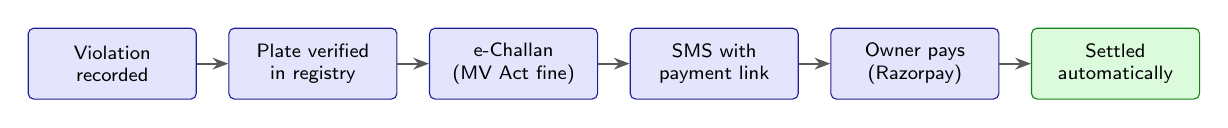
\begin{tikzpicture}[
  st/.style={draw=dBlue,fill=fBlue,rounded corners=2pt,align=center,font=\scriptsize,minimum height=9mm,text width=19mm},
  ok/.style={draw=dGreen,fill=fGreen,rounded corners=2pt,align=center,font=\scriptsize,minimum height=9mm,text width=19mm},
  ar/.style={-{Stealth[length=2mm]},thick,gray!70!black}]
\node[st] (a) at (0,0) {Violation\\recorded};
\node[st,right=4mm of a] (b) {Plate verified\\in registry};
\node[st,right=4mm of b] (c) {e-Challan\\(MV Act fine)};
\node[st,right=4mm of c] (d) {SMS with\\payment link};
\node[st,right=4mm of d] (e) {Owner pays\\(Razorpay)};
\node[ok,right=4mm of e] (f) {Settled\\automatically};
\foreach \x/\y in {a/b,b/c,c/d,d/e,e/f} \draw[ar] (\x) -- (\y);
\end{tikzpicture}
\vspace{0.5em}
\begin{columns}[T,onlytextwidth]
\begin{column}{0.48\textwidth}
\hd{\small How payment is confirmed}
\scriptsize
\begin{itemize}\setlength{\itemsep}{0.15em}
  \item Notice goes by SMS with a payment link.
  \item Payment is confirmed by a signed redirect, a signed webhook and periodic reconciliation with the gateway,
        and settlement is \textbf{idempotent}.
  \item Payment clears every block automatically; no money is ever deducted without the owner's consent.
  \item Deployment prerequisites: DLT-registered SMS and a government payment gateway; the demonstration uses
        test-mode Razorpay and an Android SMS gateway.
\end{itemize}
\end{column}
\begin{column}{0.49\textwidth}
\hd{\small Verified on the deployed system (test mode)}
\scriptsize
\begin{itemize}\setlength{\itemsep}{0.15em}
  \item A Rs~1500 challan was paid through the Razorpay test gateway and settled automatically, its stored payment
        identifier matching the gateway record.
  \item Challan notices with a live payment link reached an allow-listed team phone through an Android SMS gateway,
        while 119 pre-existing challans were correctly not texted.
  \item The automated test suite (gateways mocked, database copies only) covers these paths.
\end{itemize}
\end{column}
\end{columns}
\end{frame}

%------------------------ 10(b). ENFORCEMENT POLICY --------------------
\begin{frame}{10(b). ENFORCEMENT -- PENALTIES \& REPEAT OFFENDERS}
\begin{columns}[T,onlytextwidth]
\begin{column}{0.44\textwidth}
\hd{\small Statutory penalties (MV (Amendment) Act 2019 [26])}\\[0.2em]
\scriptsize
\begin{tabular}{@{}llp{30mm}@{}}
\toprule
\textbf{Violation} & \textbf{Section} & \textbf{Penalty}\\
\midrule
No helmet & s.~194D & Rs~1000 + three-month disqualification\\
Triple-riding & s.~194C & Rs~1000 + three months\\
No seat belt & s.~194B & Rs~1000\\
\bottomrule
\end{tabular}\\[0.6em]
\hd{\small Graduated schedule (within 365 days)}\\[0.2em]
\begin{tabular}{@{}lll@{}}
\toprule
\textbf{Offence} & \textbf{Fine} & \textbf{Licence}\\
\midrule
1st & Rs~500 & --\\
2nd & Rs~1000 & --\\
3rd & Rs~3000 & suspended\\
\bottomrule
\end{tabular}\\[0.3em]
{\tiny Whichever of the statutory and graduated fine is higher applies.}
\end{column}
\begin{column}{0.53\textwidth}
\hd{\small Rules applied to every e-challan}
\scriptsize
\begin{itemize}\setlength{\itemsep}{0.15em}
  \item A third offence, or five challans in a year, suspends the licence; the strike cycle restarts once a
        suspension ends, but no challan or suspension is ever deleted from the driver's record.
  \item Only a read that is a valid registration and is found in the vehicle registry leads to an automatic
        challan; a missing, malformed or unregistered plate is not fined but placed before an officer with the
        reason recorded.
  \item The registry is the system's own table of registered vehicles, behind a provider interface to which a
        Vahan/RC lookup can be attached without code change.
  \item A plausibility hold prevents any reading above 200 km/h from becoming a penalty: such a reading is marked
        disputed and sent to an officer.
\end{itemize}
\hd{\small Verified on the deployed system}
\begin{itemize}\setlength{\itemsep}{0.15em}
  \item A test vehicle accumulated Rs~500, Rs~1000 and Rs~3000 challans and a licence suspension, each with its SMS.
  \item A 367.6 km/h reading on the deployed system was held and its suspension lifted with an audit trail.
\end{itemize}
\end{column}
\end{columns}
\end{frame}

%------------------------ 10(c). UNPAID CHALLAN ESCALATION ------------
\begin{frame}{10(c). UNPAID E-CHALLANS -- ESCALATION (INDIAN PROCEDURE)}
\centering
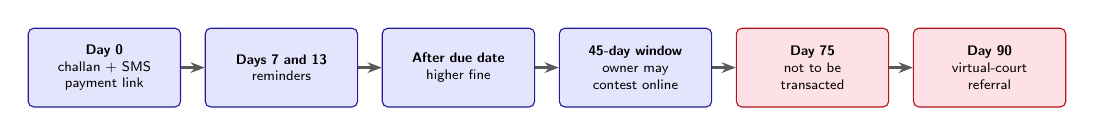
\begin{tikzpicture}[
  st/.style={draw=dBlue,fill=fBlue,rounded corners=2pt,align=center,font=\tiny,minimum height=10mm,text width=17mm},
  bad/.style={draw=dRed,fill=fRed,rounded corners=2pt,align=center,font=\tiny,minimum height=10mm,text width=17mm},
  ar/.style={-{Stealth[length=1.8mm]},thick,gray!70!black}]
\node[st] (a) at (0,0) {\textbf{Day 0}\\challan + SMS\\payment link};
\node[st,right=3mm of a] (b) {\textbf{Days 7 and 13}\\reminders};
\node[st,right=3mm of b] (c) {\textbf{After due date}\\higher fine};
\node[st,right=3mm of c] (d) {\textbf{45-day window}\\owner may\\contest online};
\node[bad,right=3mm of d] (e) {\textbf{Day 75}\\not to be\\transacted};
\node[bad,right=3mm of e] (f) {\textbf{Day 90}\\virtual-court\\referral};
\foreach \x/\y in {a/b,b/c,c/d,d/e,e/f} \draw[ar] (\x) -- (\y);
\end{tikzpicture}
\vspace{0.6em}
\begin{columns}[T,onlytextwidth]
\begin{column}{0.5\textwidth}
\hd{\small How a non-payer is handled}
\scriptsize
\begin{itemize}\setlength{\itemsep}{0.15em}
  \item Unpaid challans follow a schedule modelled on Indian e-challan procedure: reminders on days 7 and 13, a
        higher fine after the due date, a 45-day window in which the owner may contest online.
  \item A ``not to be transacted'' block on the vehicle at day 75, with a live alert if any camera sees it again.
  \item Referral to a virtual court at day 90.
  \item Payment clears every block automatically; no money is ever deducted without the owner's consent.
\end{itemize}
\end{column}
\begin{column}{0.47\textwidth}
\hd{\small Observed on the deployed system}
\scriptsize
\begin{itemize}\setlength{\itemsep}{0.15em}
  \item On the real records, the unpaid-challan schedule marked \textbf{7} vehicles not to be transacted and
        referred \textbf{8} challans to court.
  \item Its first run sent no burst of old reminders.
\end{itemize}
\end{column}
\end{columns}
\end{frame}

%------------------------ 11. EVALUATION METRICS ----------------------
\begin{frame}{11. RESULTS \& EVALUATION -- EVALUATION METRICS}
\scriptsize
\begin{columns}[T,onlytextwidth]
\begin{column}{0.49\textwidth}
\begin{itemize}\setlength{\itemsep}{0.35em}
  \item \textbf{Detection.} Precision, recall and mAP at IoU 0.5 and averaged over IoU 0.5--0.95; their divergence
        measures localisation tightness.
  \item \textbf{Tracking.} MOTA [8]:\\[0.2em]
        $\text{MOTA}=1-\dfrac{\sum_t(\mathrm{FN}_t+\mathrm{FP}_t+\mathrm{IDSW}_t)}{\sum_t\mathrm{GT}_t}$\\[0.3em]
        IDF1 [9], the F1 score over identity-matched detections, which best captures whether a vehicle keeps one
        identity throughout its visibility --- the property violation aggregation depends on; HOTA [10]; and the raw
        identity-switch count IDSW, computed with the reference TrackEval implementation.
  \item \textbf{Gate.} The false-issuance rate: automatically issued events a reviewer judged unsupported, divided by
        automatically issued events.
\end{itemize}
\end{column}
\begin{column}{0.48\textwidth}
\begin{itemize}\setlength{\itemsep}{0.35em}
  \item \textbf{ANPR.} Exact-match accuracy over the full plate string, character error rate (Levenshtein edits per
        true character) and no-read rate, with localisation scored separately so detector and OCR failures are not
        conflated.
  \item \textbf{Accidents.} Event level: a detection is a true positive if it falls between the labelled crash start
        and 10~s after its end; anything else is a false alarm. We report crashes found, precision, false alarms per
        hour of video and the mean time from impact to alert.
  \item \textbf{Fog.} ROC AUC of the fog score for fog versus clear, at clip and frame level, and the accuracy of the
        deployed visibility grades.
\end{itemize}
\vspace{0.4em}
\begin{beamercolorbox}[sep=0.5em,rounded=true]{block body}
\scriptsize Every figure is measured, with the producing data named; what is not yet measured is stated as future
work. A raw detector confidence is never reported as an accuracy.
\end{beamercolorbox}
\end{column}
\end{columns}
\end{frame}

%------------------------ 11. DETECTION PERFORMANCE -------------------
\begin{frame}{11. RESULTS \& EVALUATION -- DETECTION PERFORMANCE}
\begin{columns}[T,onlytextwidth]
\begin{column}{0.63\textwidth}
\scriptsize
{\tiny Table 2: Detector validation metrics, read from the \texttt{train\_metrics} block of each checkpoint. The last
column is the fraction of mAP@50 retained at the stricter IoU sweep --- a measure of localisation tightness.}\\[0.2em]
\setlength{\tabcolsep}{2.4pt}
\begin{tabular}{@{}lccccc@{}}
\toprule
\textbf{Detector} & \textbf{Prec.} & \textbf{Recall} & \textbf{mAP@50} & \textbf{mAP@50:95} & \textbf{Retained}\\
\midrule
Helmet (YOLOv8s) & 0.852 & 0.812 & 0.852 & 0.374 & 44\%\\
Seat belt (YOLOv8s) & 0.981 & 0.971 & 0.984 & 0.649 & 66\%\\
Two-wheeler (YOLOv8n) & 0.837 & 0.822 & 0.868 & 0.561 & 65\%\\
Plate, deployed (YOLOv8n) & 0.983 & 0.936 & 0.966 & 0.672 & 70\%\\
Plate, alternative & 0.950 & 0.893 & 0.940 & 0.463 & 49\%\\
\midrule
Per-class breakdown & \multicolumn{5}{l}{future work (re-run \texttt{yolo val} on recovered corpora)}\\
Mean $\pm$ s.d.\ over seeds & \multicolumn{5}{l}{future work (one training run per model)}\\
\bottomrule
\end{tabular}
\vspace{0.4em}
\begin{itemize}\setlength{\itemsep}{0.1em}
  \item At IoU 0.5 three of the four detectors sit between 0.85 and 0.98.
  \item The helmet detector retains only \textbf{44\%} of its mAP@50 at the stricter sweep --- it locates helmets
        reliably and draws them loosely --- while the plate detector retains \textbf{70\%}.
  \item Three downstream stages consume crops rather than boxes: the helmet verdict comes from a head-region crop, the
        seat-belt verdict from an occupant region, and OCR from the plate crop. A loose box yields a misaligned crop.
\end{itemize}
\end{column}
\begin{column}{0.35\textwidth}
\centering
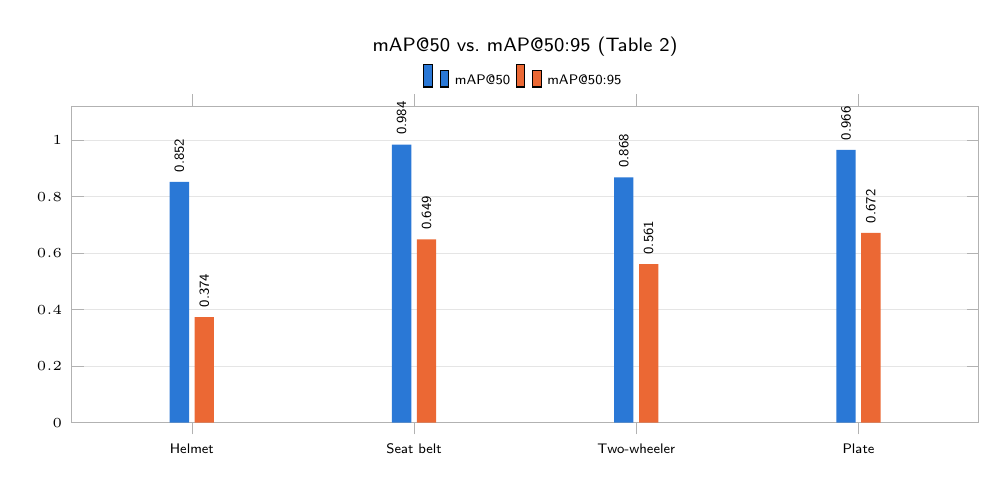
\begin{tikzpicture}
\begin{axis}[
  width=1.08\linewidth, height=5.6cm,
  ybar, bar width=7pt, ymin=0, ymax=1.12,
  enlarge x limits=0.18,
  symbolic x coords={Helmet,Seat belt,Two-wheeler,Plate},
  xtick=data, xticklabel style={font=\tiny},
  yticklabel style={font=\tiny}, ytick={0,0.2,0.4,0.6,0.8,1},
  axis line style={gray!60}, tick style={gray!60},
  ymajorgrids, grid style={gray!20},
  nodes near coords, point meta=explicit symbolic,
  every node near coord/.append style={font=\fontsize{4.6}{5}\selectfont,rotate=90,anchor=west},
  legend style={font=\tiny,at={(0.5,1.02)},anchor=south,legend columns=2,draw=none},
  title={\scriptsize mAP@50 vs.\ mAP@50:95 (Table 2)}, title style={yshift=3mm}]
\addplot[fill=sBlue,draw=none] coordinates {(Helmet,0.852) [0.852] (Seat belt,0.984) [0.984] (Two-wheeler,0.868) [0.868] (Plate,0.966) [0.966]};
\addplot[fill=sOrange,draw=none] coordinates {(Helmet,0.374) [0.374] (Seat belt,0.649) [0.649] (Two-wheeler,0.561) [0.561] (Plate,0.672) [0.672]};
\legend{mAP@50,mAP@50:95}
\end{axis}
\end{tikzpicture}
\end{column}
\end{columns}
\end{frame}

%------------------------ 11. THROUGHPUT ------------------------------
\begin{frame}{11. RESULTS \& EVALUATION -- RUNTIME THROUGHPUT}
\begin{columns}[T,onlytextwidth]
\begin{column}{0.5\textwidth}
\centering
{\tiny Table 3: Throughput on an idle laptop CPU, 200 frames per clip.}\\[0.2em]
\scriptsize
\begin{tabular}{@{}lcc@{}}
\toprule
\textbf{Clip} & \textbf{FPS} & \textbf{FPS + OCR}\\
\midrule
seatbelt.mp4 ($1280\times720$) & 1.66 & 1.07\\
seat\_belt\_video\_1 ($1280\times720$) & 1.14 & 0.37\\
triple\_riding\_video\_1 ($640\times480$) & 1.01 & 0.36\\
road traffic ($1920\times1080$, 60 FPS) & 0.91 & 0.52\\
seat\_belt\_video\_2 ($1280\times720$) & 0.26 & 0.11\\
\bottomrule
\end{tabular}
\end{column}
\begin{column}{0.47\textwidth}
\scriptsize
\begin{itemize}\setlength{\itemsep}{0.3em}
  \item Measured on an idle laptop CPU over 200 frames per clip with all five detectors resident.
  \item Plate OCR (EasyOCR at the time of measurement) costs two to three times the throughput.
  \item Cost follows scene density, not resolution --- two $1280\times720$ clips differ by \textbf{4.4$\times$}.
  \item At \textbf{0.26--1.66 FPS} the deployed CPU configuration is one to two orders of magnitude below the
        25--60 FPS of the source material, and \textbf{no real-time claim is made}.
  \item The plate-specific recogniser reads a plate about ten times faster than EasyOCR.
\end{itemize}
\end{column}
\end{columns}
\end{frame}

%------------------------ 11. TRACKING --------------------------------
\begin{frame}{11. RESULTS \& EVALUATION -- TRACKING}
\scriptsize
\centering
{\tiny Table 4: Multi-object tracking on ten UA-DETRAC sequences, identical cached YOLOv8 detections for every tracker.
The last column is per-sequence IDF1, mean $\pm$ s.d.}\\[0.2em]
\setlength{\tabcolsep}{4pt}
\begin{tabular}{@{}lcccccc@{}}
\toprule
\textbf{Tracker} & \textbf{MOTA}$\uparrow$ & \textbf{IDF1}$\uparrow$ & \textbf{HOTA}$\uparrow$ & \textbf{IDSW}$\downarrow$ & \textbf{FPS}$\uparrow$ & \textbf{IDF1/seq}\\
\midrule
\textbf{ByteTrack} (deployed) & 67.5 & \textbf{75.2} & 61.0 & \textbf{451} & 357 & 74.1$\pm$11.3\\
Centroid (fallback) & 68.3 & 68.2 & 58.9 & 1583 & 4266 & 67.5$\pm$10.7\\
DeepSORT [5] & 68.7 & 74.3 & 61.5 & 718 & $\approx$1 & 74.1$\pm$8.4\\
No tracker & $-$6.7 & 0.7 & 6.0 & 93\,053 & -- & 0.9$\pm$0.8\\
\bottomrule
\end{tabular}
\vspace{0.6em}
\raggedright
\begin{itemize}\setlength{\itemsep}{0.2em}
  \item The deployed tracker is ByteTrack [6], invoked through the Ultralytics interface; the centroid associator is the
        fallback, and DeepSORT [5] is implemented as a comparison baseline. One cached detection stream per sequence was
        replayed through every tracker, including a per-frame baseline with no association.
  \item ByteTrack keeps identities markedly better than centroid association: IDF1 is \textbf{6.65 points higher}
        (paired $t$-test, $p_\mathrm{Holm}=0.003$) with \textbf{3.5$\times$ fewer identity switches}.
  \item Against DeepSORT the IDF1 difference is $-0.02$ points and not significant ($p_\mathrm{Holm}=0.99$), while
        DeepSORT's appearance network makes association about \textbf{357$\times$ slower}.
  \item MOTA differences between the three trackers are not significant (all $p_\mathrm{Holm}\geq0.58$): MOTA is
        dominated by detection quality, which is shared.
  \item ByteTrack is the right default for violation aggregation.
\end{itemize}
\end{frame}

%------------------------ 11. SPEED -----------------------------------
\begin{frame}{11. RESULTS \& EVALUATION -- SPEED ESTIMATION}
\begin{columns}[T,onlytextwidth]
\begin{column}{0.5\textwidth}
\scriptsize
\begin{itemize}\setlength{\itemsep}{0.25em}
  \item Speed derives from tracked displacement (Equation~1). The same estimator was applied to tracker trajectories
        and to ground-truth trajectories on UA-DETRAC with the same scale: the mean absolute difference is
        \textbf{3.00 km/h} for ByteTrack, 3.93 for DeepSORT and 4.01 for centroid association; 0.16\% of ByteTrack
        estimates exceed 200 km/h.
  \item On the project footage, across 21\,726 recorded estimates the mean is 12.06 km/h and the maximum
        781.68 km/h; in a 60 km/h zone 402 estimates exceed the limit, of which 29 exceed 200 km/h.
  \item Those are artefacts of three separable mechanisms: identity switches, the single uncalibrated scale constant,
        and the frame rate fixed at 25.0 FPS, which scales every speed on 59.94 FPS material by
        $25/59.94\approx0.42$.
  \item The plausibility hold now keeps such readings out of enforcement --- a 367.6 km/h reading on the deployed
        system was held and its suspension lifted with an audit trail.
  \item Absolute accuracy against a field reference (GPS or radar) is future work; the protocol and scoring script
        are ready.
\end{itemize}
\end{column}
\begin{column}{0.47\textwidth}
\centering
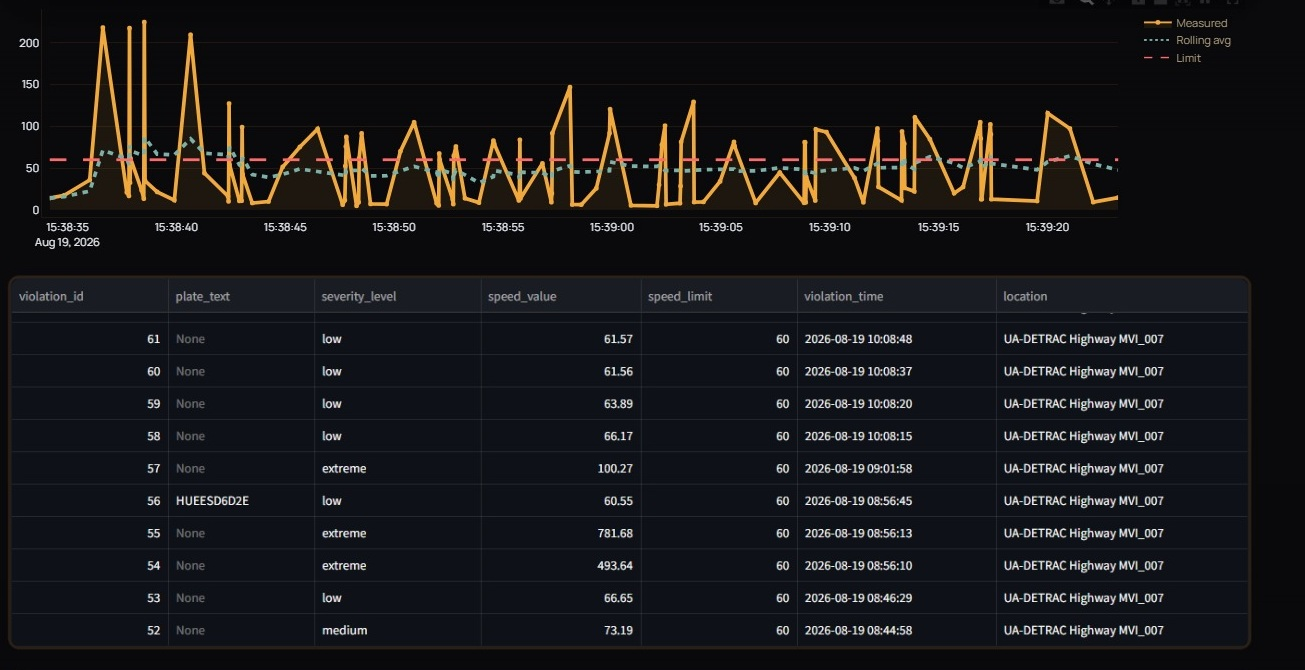
\includegraphics[width=\linewidth,height=0.5\textheight,keepaspectratio]{fig3_speed_failure.jpg}\\[0.2em]
{\tiny Fig.~3: Failure case, retained deliberately rather than omitted: speed telemetry against the 60 km/h limit, in
which the excursions above 200 km/h are artefacts of tracking and calibration rather than vehicles. Such readings are
now held for review instead of fined.\par}
\end{column}
\end{columns}
\end{frame}

%------------------------ 11. ANPR ------------------------------------
\begin{frame}{11. RESULTS \& EVALUATION -- ANPR}
\begin{columns}[T,onlytextwidth]
\begin{column}{0.52\textwidth}
\centering
{\tiny Table 5: ANPR on 291 held-out Indian plate photos (scored once). Exact = full string match; CER = character
error rate.}\\[0.2em]
\scriptsize
\setlength{\tabcolsep}{2.4pt}
\begin{tabular}{@{}lcccc@{}}
\toprule
\textbf{Reader} & \textbf{Exact} & \textbf{+ format} & \textbf{CER} & \textbf{s/plate}\\
\midrule
Legacy cascade + EasyOCR & 7.2\% & -- & -- & --\\
YOLOv8 plate + EasyOCR & 8.2\% & 16.5\% & 0.446 & 3.0\\
\textbf{YOLOv8 plate + fast-plate-ocr} & \textbf{32.3\%} & \textbf{36.8\%} & \textbf{0.215} & \textbf{0.14--0.29}\\
fast-plate-ocr + EasyOCR backup & 32.3\% & 36.8\% & 0.209 & 2.2\\
\midrule
Plate localisation recall & \multicolumn{4}{l}{99.3\% (289 / 291)}\\
\bottomrule
\end{tabular}
\vspace{0.5em}
\raggedright
\hd{\small Error analysis (300 development photos)}
\begin{itemize}\setlength{\itemsep}{0.1em}
  \item The original reader (YOLOv8 plate box, EasyOCR) found the plate in 98.7\% of photos but read only 8.0\%
        exactly (15.0\% after format decoding).
  \item Of the wrong reads, about half had characters missing, a quarter had the state code wrong, and 11\% returned
        nothing. Fragments are now joined in reading order and the crop padded at the sides; EasyOCR was replaced by a
        plate-specific recogniser [24].
\end{itemize}
\end{column}
\begin{column}{0.45\textwidth}
\hd{\small Held-out result}
\scriptsize
\begin{itemize}\setlength{\itemsep}{0.2em}
  \item Plate localisation generalises (\textbf{99.3\%}). Reading is the bottleneck.
  \item The plate-specific recogniser more than doubles exact matches (\textbf{16.5\% $\rightarrow$ 36.8\%}), halves
        the character error rate and cuts no-reads from 11.0\% to 1.7\%, at roughly a tenth of the time per plate.
  \item Using EasyOCR as a per-plate backup adds nothing to exact matches at 7.5$\times$ the cost, so it is kept only as
        a fallback when the recogniser is missing.
  \item The recogniser's public training data does not include Indian plates, which leaves fine-tuning on Indian
        plates as the obvious next gain.
  \item A challan is issued automatically only when the read is a valid registration found in the registry.
  \item Plate crops from the wide-angle CCTV clips were below human-readable resolution, so ANPR presupposes a dedicated
        HD plate camera, with wide views routed to officer confirmation.
\end{itemize}
\end{column}
\end{columns}
\end{frame}

%------------------------ 11. GATE & ABLATION -------------------------
\begin{frame}{11. RESULTS \& EVALUATION -- GATE \& ABLATION}
\begin{columns}[T,onlytextwidth]
\begin{column}{0.47\textwidth}
\centering
{\tiny Table 6: The disagreement gate on 1204 two-wheeler crops, with human review of every event an OR rule would
fine.}\\[0.2em]
\scriptsize
\begin{tabular}{@{}lr@{}}
\toprule
\textbf{Outcome} & \textbf{Count}\\
\midrule
Both models positive $\rightarrow$ challan & 95\\
Models disagree $\rightarrow$ officer review & 191\\
Both negative $\rightarrow$ no action & 918\\
\midrule
Reviewed events (5 unclear excluded) & 281\\
Wrong automatic challans, \textbf{with gate} & \textbf{1 / 94 = 1.1\%}\\
Wrong automatic challans, OR rule & 59 / 281 = 21.0\%\\
Withheld events that were real violations & 129 / 187\\
\bottomrule
\end{tabular}
\end{column}
\begin{column}{0.5\textwidth}
\scriptsize
\begin{itemize}\setlength{\itemsep}{0.25em}
  \item The gate withholds \textbf{66.8\%} of the challans an OR rule would issue.
  \item Human review shows what that buys: the false-issuance rate falls from \textbf{21.0\% to 1.1\%}, a
        \textbf{nineteen-fold reduction}.
  \item The cost is equally clear --- 129 of the 187 withheld events were real violations, which reach an officer
        rather than being lost.
  \item The prediction recorded in the earlier version (``if the gate does not reduce false issuance, its inclusion
        is not justified'') is thereby settled in the gate's favour.
  \item Figure~4(a) shows the full precision--recall trade-off on the same reviewed events.
\end{itemize}
\hd{\small Ablation}
\begin{itemize}\setlength{\itemsep}{0.15em}
  \item Removing association: IDF1 75.2 $\rightarrow$ 0.7 (Table 4).
  \item Reader variants of Table 5: legacy cascade, two-stage, format decoding, plate-specific recogniser.
  \item Removing violation aggregation, temporal confirmation or CLAHE requires violation-level ground truth on video
        and remains future work.
\end{itemize}
\end{column}
\end{columns}
\end{frame}

%------------------------ 11. ACCIDENT DETECTION ----------------------
\begin{frame}{11. RESULTS \& EVALUATION -- ACCIDENT DETECTION}
\begin{columns}[T,onlytextwidth]
\begin{column}{0.47\textwidth}
\centering
{\tiny Table 7: Crash detection on UCF-Crime held-out clips: 23 crashes with published timings + 23 normal clips,
0.51 h.}\\[0.2em]
\scriptsize
\setlength{\tabcolsep}{2.4pt}
\begin{tabular}{@{}lcccc@{}}
\toprule
\textbf{Detector} & \textbf{Found} & \textbf{False al./h} & \textbf{Precision} & \textbf{To alert}\\
\midrule
Trajectory rules (original) & 1/23 & 0.0 & -- & 4.7 s\\
Rules, tuned on a dev set & 3/23 & 11.8 & 0.33 & 3.2 s\\
\textbf{Learned R3D-18} & \textbf{7/23} & \textbf{3.9} & \textbf{0.78} & \textbf{2.0 s}\\
\bottomrule
\end{tabular}
\vspace{0.6em}
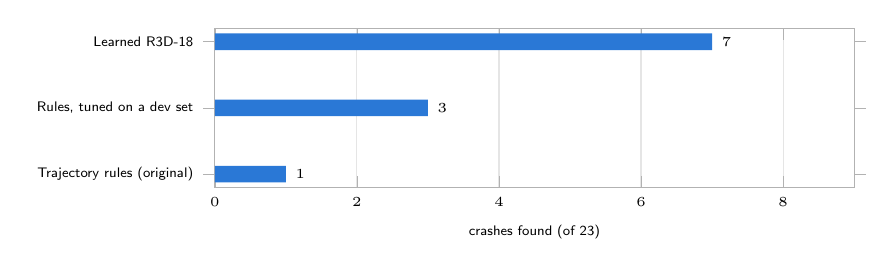
\begin{tikzpicture}
\begin{axis}[
  width=0.8\linewidth, height=3.6cm, xbar, bar width=6pt, xmin=0, xmax=9,
  symbolic y coords={A,B,C}, ytick=data, yticklabels={Trajectory rules (original),{Rules, tuned on a dev set},Learned R3D-18},
  yticklabel style={font=\tiny}, xticklabel style={font=\tiny},
  xlabel={\tiny crashes found (of 23)}, nodes near coords, every node near coord/.append style={font=\tiny},
  axis line style={gray!60}, tick style={gray!60}, xmajorgrids, grid style={gray!20}]
\addplot[fill=sBlue,draw=none] coordinates {(1,A) (3,B) (7,C)};
\end{axis}
\end{tikzpicture}
\end{column}
\begin{column}{0.5\textwidth}
\scriptsize
\begin{itemize}\setlength{\itemsep}{0.25em}
  \item The trajectory rules found 1 of 23 crashes. On $320\times240$ CCTV the detector sometimes sees no vehicle at
        all, and where it does, identities churn (one clip produced 21 track identities in 8.5~s), so cues that need
        a stable trajectory never fire.
  \item Tuning the rules on a separate development set raised recall to 3 of 23 but at 11.8 false alarms per hour.
  \item The learned video model, which needs no tracks, found \textbf{7 of 23 crashes} with 2 false alarms in
        0.51~h of video (\textbf{3.9 per hour}), precision \textbf{0.78}, alerting about 2~s after impact. It is now
        the live detector.
  \item It still misses most crashes on this footage, so alerts go to a control room that confirms before dispatch.
  \item Dispatch itself was verified: on the deployed system an alert SMS named the nearest hospital and police
        station (0.63~km each), chosen from 132 hospitals and 20 police stations imported within 5~km of the camera.
\end{itemize}
\end{column}
\end{columns}
\end{frame}

%------------------------ 11. FOG -------------------------------------
\begin{frame}{11. RESULTS \& EVALUATION -- FOG MONITORING}
\begin{columns}[T,onlytextwidth]
\begin{column}{0.45\textwidth}
\centering
{\tiny Synthetic haze added to 100 real frames}\\[0.2em]
\scriptsize
\begin{tabular}{@{}cc@{}}
\toprule
\textbf{Transmission $t$} & \textbf{Mean fog score}\\
\midrule
1.0  & 0.000\\
0.85 & 0.238\\
0.70 & 0.439\\
0.50 & 0.688\\
0.35 & 0.822\\
0.20 & 0.942\\
\bottomrule
\end{tabular}
\end{column}
\begin{column}{0.52\textwidth}
\scriptsize
\begin{itemize}\setlength{\itemsep}{0.3em}
  \item Under synthetic haze the score rises monotonically with haze density.
  \item On real footage from twenty different cameras the score separates fog from clear with \textbf{ROC AUC 0.95}
        at clip level and \textbf{0.97} at frame level.
  \item The deployed grades are conservative: every clear clip stays clear, but only 3 of the 10 fog clips reach
        ``moderate fog'', so the deployed grading is \textbf{65\% correct}.
  \item Recalibrating the grade thresholds on more real footage is a settings change; we did not tune them on these
        twenty clips, since that would make the reported figure self-confirming.
\end{itemize}
\end{column}
\end{columns}
\end{frame}

%------------------------ 11. QUALITATIVE -----------------------------
\begin{frame}{11. RESULTS \& EVALUATION -- QUALITATIVE RESULTS}
\begin{columns}[T,onlytextwidth]
\begin{column}{0.49\textwidth}
\centering
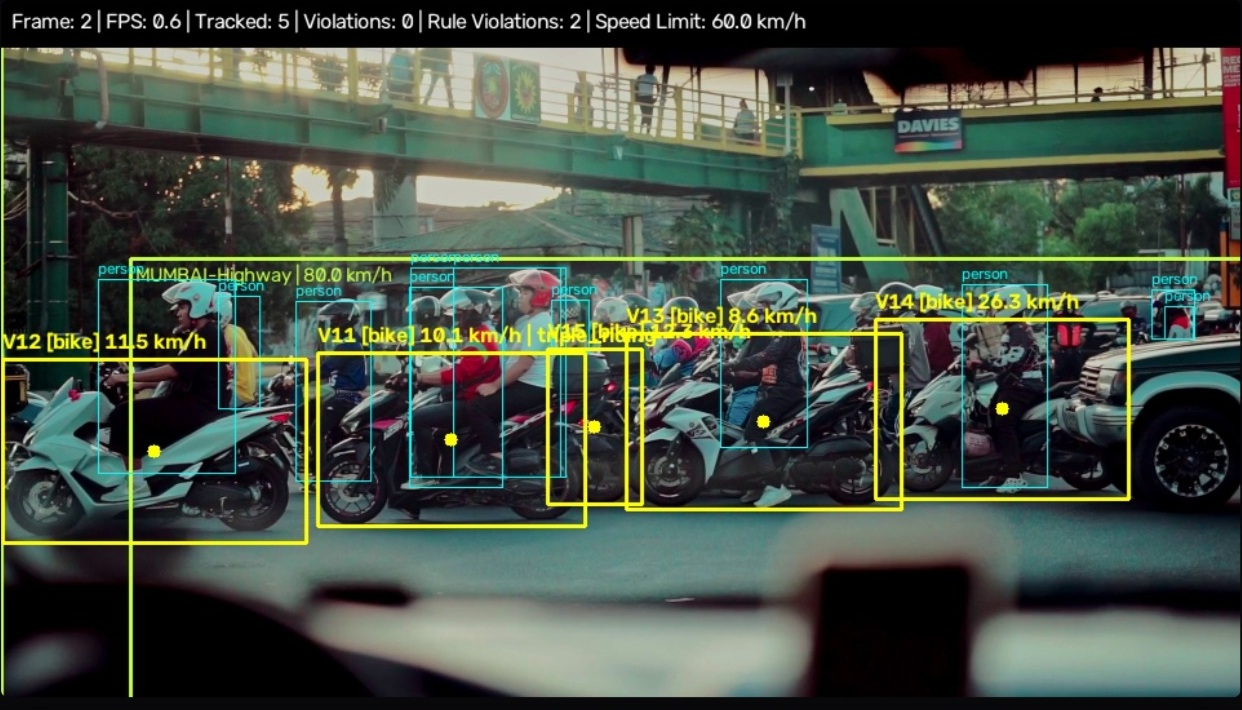
\includegraphics[width=\linewidth,height=0.5\textheight,keepaspectratio]{fig2a_dense_traffic.jpg}\\[0.2em]
{\tiny (a) Dense two-wheeler traffic: identities held under heavy mutual occlusion, with concurrent triple-riding flags
and per-vehicle speed labels.\par}
\end{column}
\begin{column}{0.49\textwidth}
\centering
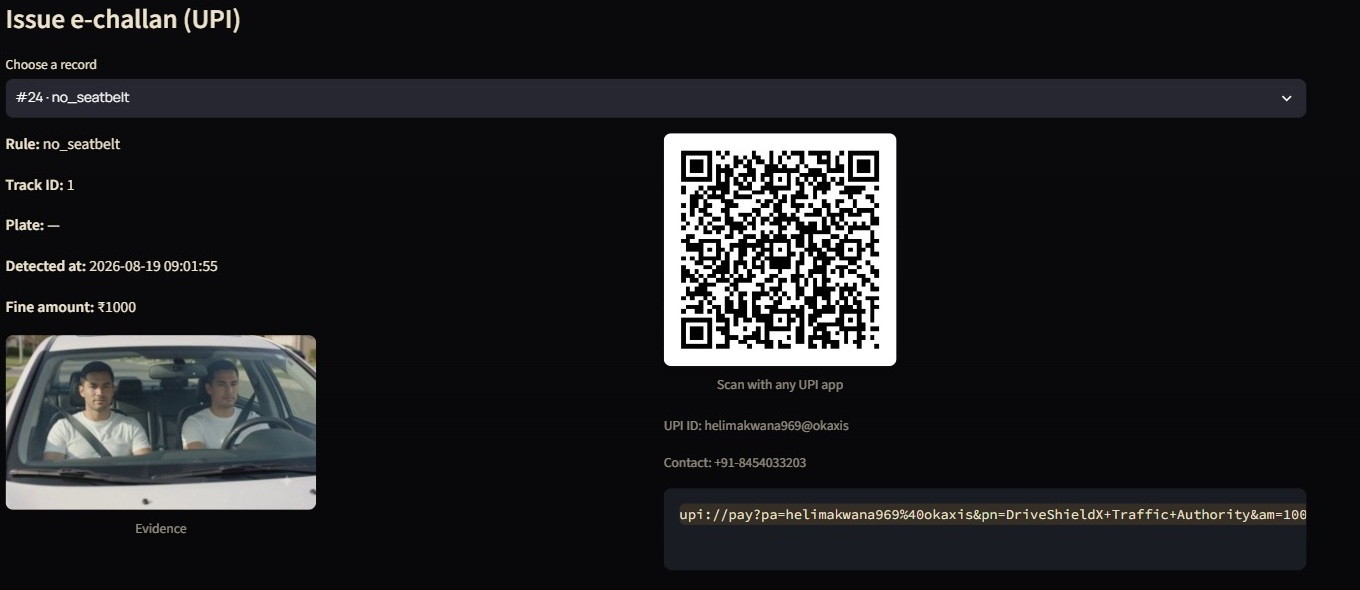
\includegraphics[width=\linewidth,height=0.5\textheight,keepaspectratio]{fig2b_seatbelt_evidence.jpg}\\[0.2em]
{\tiny (b) Seat-belt violation with its retained evidence crop. The plate field is empty; such an event is now not
issued automatically but routed to an officer.\par}
\end{column}
\end{columns}
\vspace{0.4em}
{\centering\scriptsize Fig.~2: Operation on real footage. Panel (a) is the hardest case in the set --- close-spaced
two-wheelers occluding one another --- in which identities survive and triple-riding is flagged alongside speed on the
same tracks.\par}
\end{frame}

%------------------------ 11. PR CURVES -------------------------------
\begin{frame}{11. RESULTS \& EVALUATION -- PR CURVES}
\centering
\IfFileExists{pr_curves.pdf}{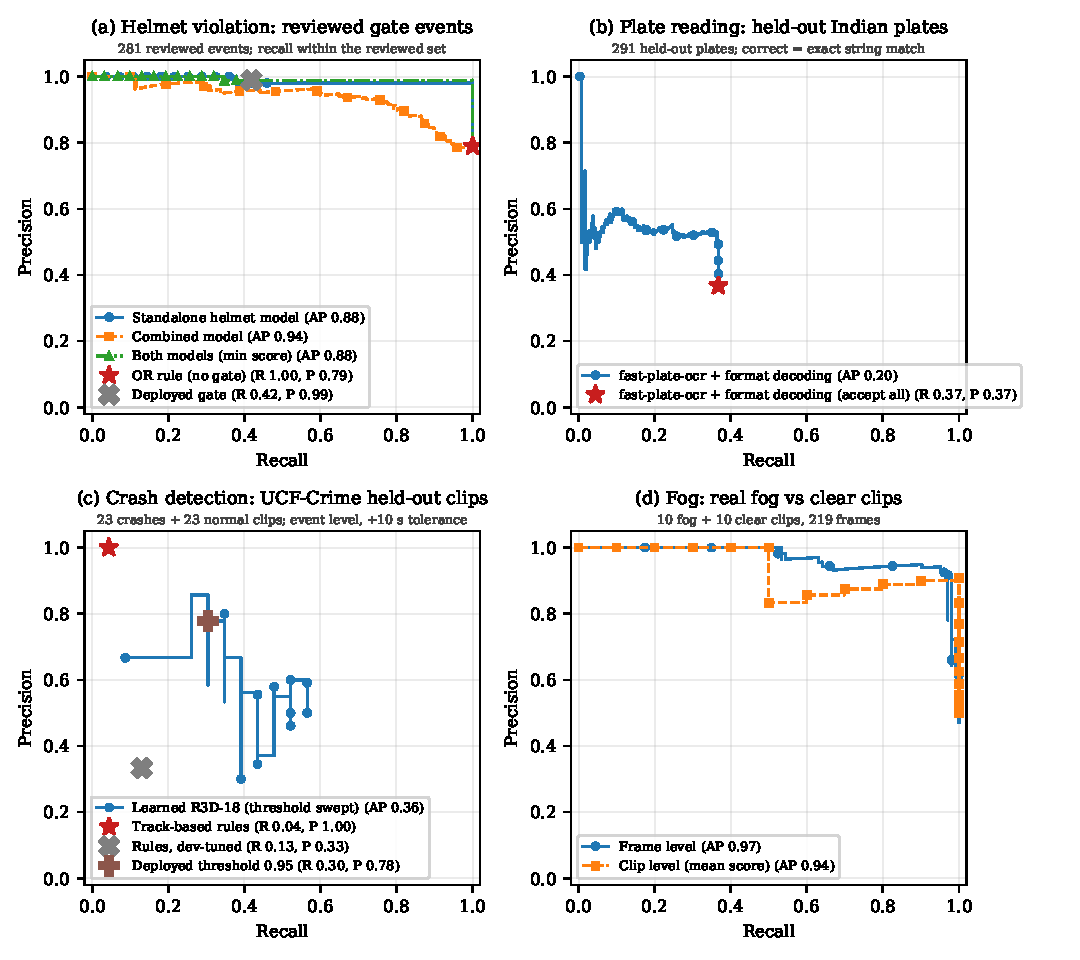
\includegraphics[width=0.62\textwidth,height=0.7\textheight,keepaspectratio]{pr_curves.pdf}}{\fbox{\parbox[c][0.6\textheight][c]{0.55\textwidth}{\centering\nm{Figure~4 is generated by \texttt{python -m evaluation.pr\_curves} from the project's labelled evaluations.}}}}\\[0.2em]
{\tiny Fig.~4: Precision versus recall on the project's labelled evaluations. (a) Helmet violation on the 281
human-reviewed gate events, scored by the standalone model, the combined model and both together; the OR rule and the
deployed gate are marked. (b) Plate reading on 291 held-out Indian plates as the confidence needed to accept a read is
raised. (c) Crash detection on the UCF-Crime held-out clips at event level as the alarm threshold is swept, with the
rule-based detectors marked. (d) Fog versus clear at frame and clip level. AP = average precision.\par}
\end{frame}

%------------------------ 12. DISCUSSION ------------------------------
\begin{frame}{12. DISCUSSION (1/2)}
\footnotesize
\begin{columns}[T,onlytextwidth]
\begin{column}{0.49\textwidth}
\hd{\small What the System Does Well}
\begin{itemize}\setlength{\itemsep}{0.2em}
  \item The contribution that survives scrutiny is now \textbf{both architectural and measured}.
  \item Four violation types are evaluated inside one inference cycle against one persistent vehicle identity, and
        ByteTrack keeps that identity with IDF1 75.2 on public ground truth --- on a par with DeepSORT at a fraction
        of the cost.
  \item The disagreement gate gives the pipeline a state published enforcement systems generally lack, and human
        review shows it removes almost all wrong automatic challans.
  \item Registry verification closes the most damaging failure of automated e-challans, the notice sent to the wrong
        citizen.
  \item Plate localisation (99.3\% on held-out photos), seat-belt detection (mAP@50 0.984) and the fog index
        (AUC 0.95) are strong in their own right.
\end{itemize}
\end{column}
\begin{column}{0.48\textwidth}
\hd{\small Comparison with Existing Approaches}
\begin{itemize}\setlength{\itemsep}{0.2em}
  \item We offer no numerical comparison against the systems surveyed in the literature review: those studies report
        on their own datasets under their own capture conditions, and a table juxtaposing our 0.852 with a
        published 0.993 would imply a comparison never performed.
  \item Against the e-challan systems already operating in India, the distinction DriveShieldX draws is in capability: one record per
        vehicle across violations, a deferral state instead of automatic issuance on a disputed prediction, no
        challan without a verified plate, repeat-offender and escalation logic that run themselves, and crash and fog
        monitoring on the same cameras.
\end{itemize}
\end{column}
\end{columns}
\end{frame}

\begin{frame}{12. DISCUSSION (2/2)}
\small
\begin{columns}[T,onlytextwidth]
\begin{column}{0.96\textwidth}
\hd{Failure Cases}
\begin{itemize}\setlength{\itemsep}{0.3em}
  \item \textbf{Reading, not finding, limits attribution.} Plates are found in 99.3\% of photos but read exactly in
        36.8\%. Unverified reads are routed to an officer, so the cost is officer time rather than wrong challans.
  \item \textbf{Crashes on low-resolution CCTV.} The learned model finds 7 of 23 held-out crashes; most are still
        missed, and the alert therefore goes to a person, not straight to an ambulance.
  \item \textbf{Loose localisation propagates} into every crop-consuming stage; the helmet detector retains only 44\%
        of its mAP@50 at mAP@50:95.
  \item \textbf{Speed is consistent but not calibrated.} Tracking adds about 3 km/h of error; the scale constant and
        the fixed frame rate dominate absolute error until per-camera calibration is done.
  \item \textbf{Throughput.} 0.26--1.66 FPS on a CPU is far from multi-camera real time.
\end{itemize}
\end{column}
\end{columns}
\end{frame}

%------------------------ 13. APPLICATIONS ----------------------------
\begin{frame}{13. APPLICATIONS}
\small
\vspace{0.3em}
\begin{columns}[T,onlytextwidth]
\begin{column}{0.31\textwidth}
\begin{block}{Traffic Authority Dashboard}
Violations with their evidence crops; the officer review queue for events the gate withholds and plates that cannot
be verified.
\end{block}
\begin{block}{Vehicle Owner}
SMS notice with a payment link; self-settling online payment; a 45-day window to contest online.
\end{block}
\end{column}
\begin{column}{0.31\textwidth}
\begin{block}{Police Department}
Accident alerts with the nearest police station, distance and map links; a live alert when a vehicle marked not to be
transacted is seen again.
\end{block}
\begin{block}{Hospital / Ambulance}
The nearest hospital, located from the camera's GPS position and OpenStreetMap data.
\end{block}
\end{column}
\begin{column}{0.31\textwidth}
\begin{block}{Road-Safety Zones}
A sustained moderate or dense fog grade raises a zone advisory.
\end{block}
\begin{block}{Analytics \& Heatmaps}
Cities have installed CCTV by the thousand; the same feeds are watched continuously instead of consulted only after a
collision.
\end{block}
\end{column}
\end{columns}
\vspace{0.4em}
{\centering\color{dsblue}\textbf{The action layer of Fig.~1: authority, owner, police, hospital and analytics.}\par}
\end{frame}

%------------------------ 14. LIMITATIONS & FUTURE WORK ---------------
\begin{frame}{14. LIMITATIONS AND FUTURE WORK}
\begin{columns}[T,onlytextwidth]
\begin{column}{0.53\textwidth}
\hd{\small Limitations and Outstanding Work}
\scriptsize
\begin{itemize}\setlength{\itemsep}{0.15em}
\item \textbf{Training corpora are not in hand.} Until they are recovered, no per-class precision, recall or F1 can be
reported for the detectors, and no dataset size or class balance can be stated.
\item \textbf{One training run per detector.} Mean $\pm$ standard deviation requires a seed sweep.
\item \textbf{Violation-level accuracy on video} for helmet, triple-riding and seat belt, and the ablations that depend
on it (aggregation, temporal confirmation, CLAHE), still need labelled video.
\item \textbf{Speed} needs per-zone calibration, the true frame rate read from the stream, and a field check against GPS
or radar.
\item \textbf{Plate reading} would benefit from fine-tuning the recogniser on Indian plates and from HD plate cameras.
\item \textbf{Crash detection} needs more and more varied training crashes than the 127 labelled here.
\item \textbf{Deployment prerequisites.} Official Vahan/Sarathi/Parivahan access (through NIC), DLT-registered SMS and
a government payment gateway; the demonstration uses test-mode Razorpay and an Android SMS gateway. Continuous
processing of public video carries data-protection obligations under the DPDP Act 2023: retention limits, access
control and an appeal route, which the contest window and officer review partly provide.
\end{itemize}
\end{column}
\begin{column}{0.44\textwidth}
\hd{\small Future Work}
\scriptsize
\begin{enumerate}\setlength{\itemsep}{0.25em}
  \item Recover the corpora and re-validate per class.
  \item Fine-tune plate reading on Indian plates.
  \item Calibrate speed per camera against a field reference.
  \item Enlarge the crash training set.
  \item Measure violation-level accuracy on labelled video.
  \item Only then do red-light and wrong-way violations, cross-camera identity fusion and quantised edge deployment
        become worth pursuing.
\end{enumerate}
\end{column}
\end{columns}
\end{frame}

%------------------------ 15. CONCLUSION ------------------------------
\begin{frame}{15. CONCLUSION}
\small
\begin{itemize}\setlength{\itemsep}{0.45em}
  \item DriveShieldX monitors road-safety violations with a \textbf{single detection and tracking pipeline}, binds
        every flag to \textbf{one persistent vehicle identity}, and carries the record through plate reading and
        registry verification to an automated challan, declining to issue when two models disagree or the plate
        cannot be verified.
  \item Measured on independent ground truth, ByteTrack holds identities at \textbf{IDF1 75.2}, the gate cuts wrong
        automatic challans from \textbf{21.0\% to 1.1\%}, plate localisation reaches \textbf{99.3\%} and exact reading
        \textbf{36.8\%}, a learned crash model finds \textbf{seven times as many} held-out crashes as the trajectory
        rules it replaces, and the fog index separates fog from clear footage with \textbf{AUC 0.95}.
  \item Its boundaries are equally clear: plate reading and crash recall are the weakest stages, CPU throughput is
        0.26--1.66 FPS, and the speed scale is uncalibrated.
\end{itemize}
\end{frame}

%------------------------ ACKNOWLEDGEMENT -----------------------------
\begin{frame}{ACKNOWLEDGEMENT}
\small
\vspace{0.5em}
We express our sincere gratitude to our project guide \textbf{Prof. Sonal Kadam} for her valuable guidance,
constant support and feedback throughout this work.

\vspace{0.6em}
We thank \textbf{Prof. Kumud Wasnik}, Head of Department, Computer Science and Technology, for her guidance and support.

\vspace{0.6em}
The authors thank the Department of Computer Science and Technology, Usha Mittal Institute of Technology, SNDT Women's
University, for the guidance and resources provided during this work. DriveShieldX continues an earlier system,
OverSpeedX, from which the UA-DETRAC material is retained.

\vspace{1.2em}
\begin{flushright}
\begin{tabular}{@{}ll@{}}
Heli Makwana & \rollHeli\\
Nisha Mandal & \rollNisha\\
Tanisha Sankhe & \rollTanisha\\
\end{tabular}
\end{flushright}
\end{frame}

%------------------------ REFERENCES (verbatim from the paper) ------
\begin{frame}{REFERENCES (1/3)}
\scriptsize
\begin{enumerate}\setlength{\itemsep}{0.05em}
\item[{[1]}] Ultralytics, ``YOLOv8 documentation,'' 2023. https://docs.ultralytics.com
\item[{[2]}] K.\,D.\ Dharmasaputra, B.\,P.\ Hartato, et al., ``Evaluation of YOLOv8 and centroid tracking in vehicle detection, classification, and counting system,'' Int.\ J.\ Intell.\ Syst.\ Appl., Oct.\ 2025.
\item[{[3]}] S.\ Joshi, P.\ Jejure, C.\ Jadhav, and V.\ Jankar, ``Automatic number plate recognition using YOLOv8 model,'' Int.\ J.\ Sci.\ Res.\ Sci.\ Technol., 2025.
\item[{[4]}] R.\ Srinath, J.\ Vrindavanam, S.\,Y.\,R., Y.\,L., and S.\,S.\ Chegaraddi, ``Smart vehicle recognition and e-challan generation system,'' Proc.\ INCET, 2020.
\item[{[5]}] N.\ Wojke, A.\ Bewley, and D.\ Paulus, ``Simple online and realtime tracking with a deep association metric,'' Proc.\ IEEE ICIP, 2017, pp.\ 3645--3649.
\item[{[6]}] Y.\ Zhang, P.\ Sun, Y.\ Jiang, D.\ Yu, Z.\ Yuan, P.\ Luo, and X.\ Wang, ``ByteTrack: Multi-object tracking by associating every detection box,'' Proc.\ ECCV, LNCS vol.\ 13682, Springer, 2022, pp.\ 1--21.
\item[{[7]}] A.\ Bewley, Z.\ Ge, L.\ Ott, F.\ Ramos, and B.\ Upcroft, ``Simple online and realtime tracking,'' Proc.\ IEEE ICIP, 2016, pp.\ 3464--3468.
\item[{[8]}] K.\ Bernardin and R.\ Stiefelhagen, ``Evaluating multiple object tracking performance: The CLEAR MOT metrics,'' EURASIP J.\ Image Video Process., vol.\ 2008, pp.\ 1--10, 2008.
\item[{[9]}] E.\ Ristani, F.\ Solera, R.\ Zou, R.\ Cucchiara, and C.\ Tomasi, ``Performance measures and a data set for multi-target, multi-camera tracking,'' Proc.\ ECCVW, 2016, pp.\ 17--35.
\item[{[10]}] J.\ Luiten, A.\ O\v{s}ep, P.\ Dendorfer, P.\ Torr, A.\ Geiger, L.\ Leal-Taix\'e, and B.\ Leibe, ``HOTA: A higher order metric for evaluating multi-object tracking,'' Int.\ J.\ Comput.\ Vis., vol.\ 129, no.\ 2, pp.\ 548--578, 2021.
\end{enumerate}
\end{frame}
\begin{frame}{REFERENCES (2/3)}
\scriptsize
\begin{enumerate}\setlength{\itemsep}{0.05em}
\item[{[11]}] A.\ Milan, L.\ Leal-Taix\'e, I.\ Reid, S.\ Roth, and K.\ Schindler, ``MOT16: A benchmark for multi-object tracking,'' arXiv:1603.00831, 2016.
\item[{[12]}] C.-J.\ Lin and J.-Y.\ Jhang, ``Intelligent traffic-monitoring system based on YOLO and convolutional fuzzy neural networks,'' IEEE Access, vol.\ 10, pp.\ 14120--14133, 2022.
\item[{[13]}] A.\,G.\ Suman, A.\,G., G.\ Raviteja, and G.\,R., ``An efficient deep learning model for helmet detection in real-world scenarios,'' Proc.\ ICSFT, 2026.
\item[{[14]}] S.\ Sutikno, A.\ Sugiharto, and R.\ Kusumaningrum, ``Automated detection of driver and passenger without seat belt using YOLOv8,'' Int.\ J.\ Adv.\ Comput.\ Sci.\ Appl., 2023.
\item[{[15]}] P.\,K.\ Gautam and S.\ Kumar, ``A centroid-based algorithm for measuring and tracking vehicle speed from a monocular camera using the YOLOv8 object detector,'' Indones.\ J.\ Electr.\ Eng.\ Comput.\ Sci., 2025.
\item[{[16]}] R.\ Kejriwal, H.\,J.\ Ritika, A.\ Arora, and Mohana, ``Vehicle detection and counting using deep learning based YOLO and deep SORT algorithm for urban traffic management system,'' Proc.\ IEEE CONECCT, 2022, pp.\ 1--6.
\item[{[17]}] M.\,R., M.\,R., R.\ Kiruthika, and G.\,S., ``Multi-task learning architecture for vehicle detection and tracking towards passenger safety and traffic violation detection,'' Proc.\ ICMLAS, 2025.
\item[{[18]}] T.\ Qamar, N.\ Bawany, J.\ Shamsi, and K.\ Zahoor, ``Vision-based accident identification in traffic videos using deep learning,'' Suranaree J.\ Sci.\ Technol., 2024.
\item[{[19]}] K.\ Zuiderveld, ``Contrast limited adaptive histogram equalization,'' in Graphics Gems IV, Academic Press, 1994, pp.\ 474--485.
\item[{[20]}] JaidedAI, ``EasyOCR,'' 2023. https://github.com/JaidedAI/EasyOCR
\end{enumerate}
\end{frame}
\begin{frame}{REFERENCES (3/3)}
\scriptsize
\begin{enumerate}\setlength{\itemsep}{0.05em}
\item[{[21]}] L.\ Wen, D.\ Du, Z.\ Cai, Z.\ Lei, M.-C.\ Chang, H.\ Qi, J.\ Lim, M.-H.\ Yang, and S.\ Lyu, ``UA-DETRAC: A new benchmark and protocol for multi-object detection and tracking,'' Comput.\ Vis.\ Image Underst., vol.\ 193, 2020.
\item[{[22]}] F.\ Wilcoxon, ``Individual comparisons by ranking methods,'' Biom.\ Bull., vol.\ 1, no.\ 6, pp.\ 80--83, 1945.
\item[{[23]}] W.\ Sultani, C.\ Chen, and M.\ Shah, ``Real-world anomaly detection in surveillance videos,'' Proc.\ IEEE CVPR, 2018, pp.\ 6479--6488.
\item[{[24]}] ankandrew, ``fast-plate-ocr: Fast and lightweight OCR for vehicle license plates,'' v1.1, MIT licence, 2026. https://github.com/ankandrew/fast-plate-ocr
\item[{[25]}] ``Number Plate Identification Dataset,'' Bapatla Engineering College, Zenodo, 2024, doi:10.5281/zenodo.13954136 (CC-BY-4.0).
\item[{[26]}] Government of India, ``The Motor Vehicles (Amendment) Act, 2019,'' Act No.\ 32 of 2019.
\item[{[27]}] D.\ Tran, H.\ Wang, L.\ Torresani, J.\ Ray, Y.\ LeCun, and M.\ Paluri, ``A closer look at spatiotemporal convolutions for action recognition,'' Proc.\ IEEE CVPR, 2018, pp.\ 6450--6459.
\item[{[28]}] W.\ Kay et al., ``The Kinetics human action video dataset,'' arXiv:1705.06950, 2017.
\item[{[29]}] K.\ He, J.\ Sun, and X.\ Tang, ``Single image haze removal using dark channel prior,'' IEEE Trans.\ Pattern Anal.\ Mach.\ Intell., vol.\ 33, no.\ 12, pp.\ 2341--2353, 2011.
\end{enumerate}
\end{frame}


%------------------------ THANK YOU -----------------------------------
\begin{frame}[c]{\phantom{T}}
\centering
{\fontsize{30}{34}\selectfont\bfseries\color{dsblue} THANK YOU}
\end{frame}

\end{document}
